%% Template for a preprint Letter or Article for submission
%% to the journal Nature.
%% Written by Peter Czoschke, 26 February 2004
%%

\documentclass[%
%superscriptaddress,
%groupedaddress,
%unsortedaddress,
%runinaddress,
%frontmatterverbose, 
%preprint,
showpacs,
%preprintnumbers,
%nofootinbib,
%nobibnotes,
%bibnotes,
 amsmath,amssymb,
 aps,
 twocolumn,
 prl,
 reprint,
%pra,
%prb,
%rmp,
%prstab,
%prstper,
floatfix,
]{revtex4-1}

\usepackage{graphicx}% Include figure files
\usepackage{dcolumn}% Align table columns on decimal point
\usepackage{bm}% bold math
%\usepackage{lineno}
\usepackage{color}
\usepackage{acronym}
\usepackage{multirow}
\usepackage{tabularx}
\usepackage{hyperref}
%\addbibresource{references.bib}
%\linenumbers % Commence numbering lines
%\usepackage{hyperref}% add hypertext capabilities
%\usepackage[mathlines]{lineno}% Enable numbering of text and display math
%\linenumbers\relax % Commence numbering lines
\hypersetup{
%--- fill inside borders ---
  colorlinks=true,        % false: boxed links; true: colored links
  linkcolor=black,         % color of internal links
  citecolor=cyan,         % color of links to bibliography
}

%% make sure you have the nature.cls and naturemag.bst files where
%% LaTeX can find them

%\bibliographystyle{authortitle}

%% Notice placement of commas and superscripts and use of &
%% in the author list

%\author{Hunter Gabbard$^{1}$, Ik Siong Heng$^1$, Chris Messenger$^1$, \\
%    Francesco Tonolini$^2$, \& Roderick Murray-Smith$^2$}

%% ----- comment commands for each of us
\newcommand{\chris}[1]{\textbf{\textcolor{green}{CHRIS: #1}}}
\newcommand{\francesco}[1]{\textbf{\textcolor{red}{FRANCESCO: #1}}}
\newcommand{\hunter}[1]{\textbf{\textcolor{blue}{HUNTER: #1}}}
\newcommand{\siong}[1]{\textbf{\textcolor{cyan}{SIONG: #1}}}
\newcommand{\rod}[1]{\textbf{\textcolor{yellow}{ROD: #1}}}

\begin{document}

\preprint{APS/123-QED}

\title{Estimating Bayesian Parameter Estimation Using Conditional Variational
Autoencoders\chris{need to have gravitational waves in the title but stay below
15 words}}

\author{Hunter Gabbard$^1$}
 \email{Corresponding author: h.gabbard.1@research.gla.ac.uk}
\author{Chris Messenger$^1$}
\author{Ik Siong Heng$^1$}
\author{Francesco Tonolini$^2$}
\author{\& Roderick Murray-Smith$^2$}

\affiliation{
 SUPA, School of Physics and Astronomy$^1$, \\
 School of Computing Science$^2$, \\
 University of Glasgow, \\
 Glasgow G12 8QQ, United Kingdom\chris{Probably want to have 2 seperate
affiliations} \\
}

\date{\today}

\maketitle

\acrodef{GW}[GW]{gravitational wave}
\acrodef{BBH}[BBH]{binary black hole}
\acrodef{SNR}[SNR]{signal-to-noise ratio}
\acrodef{PSD}[PSD]{power spectral density}
\acrodef{FFT}[FFT]{fast Fourier transform}
\acrodef{CNN}[CNN]{convolutional neural network}
\acrodef{ROC}[ROC]{receiver operator characteristic}
\acrodef{ELBO}[ELBO]{evidence lower bound}

%
% Introductory paragraph describing the content of the letter
%
% This format begins with a title of, at most, 15 words, followed by an
% introductory paragraph (not abstract) of approximately 150 words, summarizing
% the background, rationale, main results (introduced by "Here we show" or some
% equivalent phrase) and implications of the study. This paragraph should be
% referenced, as in Nature style, and should be considered part of the main
% text, so that any subsequent introductory material avoids too much redundancy
% with the introductory paragraph.
%
\textbf{ 
%
% background
%
With the beginning of the Laser Interferometer Gravitational wave
Observatory's (LIGO)\chris{use the acronym package for ALL acronyms.} and
Virgo's third observation run well under way, we are now in an era where
\ac{GW} detection is commonplace~\cite{PhysRevLett.116.061102,
PhysRevX.6.041015,PhysRevLett.119.161101}. As the sensitivity of both detectors
increases, we will see more many more detections on a weekly and even daily
basis\chris{too vague. You could actually quote numbers here}.  The current
method used to estimate the parameters of gravitational wave events is done
using a form of\chris{a form of? } Bayesian inference~\cite{1409.7215}.
%
% rationale
%
Although effective~\chris{let's not mnake enemies. The Bayesian PE that is
currently done is excellent and amazing and computes the correct result. It is
just slow.}, Bayesian inference is a computationally expensive method which can
take of order hours to weeks to complete when applied to a single GW
event\chris{again, we can get the actual numbers for this and be more specific.
Also, why does it even matter to be fast? Need to mention that the rate of
future detections will swamp current methods *and* we desperately need accurate
low latency PE for EM follow-up.  Current low latency methods are good but only
an approximation and also take O(1 min) to run}. We propose the use of a
conditional variational autoencoder (CVAE) as a computationally
inexpensive\chris{not true. It is very expensive it's just that the cost is
spent before the events are detected allowing rapid accurate and complete
Bayesian results to be shared almost instantantaneously.  We need to be very
careful here regarding what the practical bottleneck would be for an
instantaneous PE run.} alternative to this
approach~\cite{1904.06264,1812.04405}. 
%
% results
%
Here we show that a CVAE~\chris{best to
use machine learning here as opposed to an obscure acronym.} can return
posterior estimates for any~\chris{we don't show this for *any* parameter, we
show realistic but simplified cases. We assume that this is extendable to
all/any parameters.} parameter of a detected \ac{GW} event on the order of less
than $1s$~\chris{we need to measure this number.}, an immense~\chris{quantify
this even of it's just to the nearest order of magnitude.} speed-up over
current inference techniques.}

\chris{
The paragraph structure needs to be changed a bit. Here's how I see it based on
this text from the Nature guidelines - "As a guideline, the text should be
structured in broad sections (abstract, introduction, results, conclusions,
methods)." 
\begin{itemize} 
%
\item Abstract - introductory paragraph
(not abstract) of approximately 150 words, summarizing the background,
rationale, main results (introduced by "Here we show" or some equivalent
phrase) and implications of the study. It's getting there.  
%
\item introduction - this section has to expand upon what has mentioned in the
abstract background (which was only ~50 words). It needs to cover the state of
the gravitational wave field and the number of detections expected in the next
~5 years. It should briefly discuss the issue of low latency EM follow up. It
needs to cover Bayesian inference (not in too much detail) and the signal model
we are interested in here (again, not too much detail but enough for the
average Nature reader). It then needs to introduce machine learning and focus
mainly on how our scheme works. We also need to include a statement about how
the training data priors affect the result (are they really the priors?)   
%
\item results - here you would outline the process of comparison between the
standard approach and the new one. Define training and test data and how Bilby
is run on all test data for comparison. How do we then train our network. How
do we then produce results on the test data. Here you refer to results plots
but try to not make conclusion statememnts (just descriptive). Also include the
speed analysis here.  
%
\item conclusions - now draw conclusions about the quality of the comparison
results. Highlight the current limitations but also highlight the importance of
this for the GW field (multi-detector is easy, additional parameters are easy,
longer datasets may be a challenge regarding GPU memory?, we don't have to
assume a noise model if we inject training data into real noise, we do rely on
well defined signal models, EM-follow up in very low latency, can we use
transfer learning if we want to retrain, ...) End with broader statements about
inference in other fields and how this is applicable across the sciences.
%
\item methods - Everything that we couldn't fit in. Mostly validation plots.
%
\end{itemize} }

%
% Set up parameter estimation problem
%
In the standard Bayesian \ac{GW} inference approach, we assume that we are
given some observed waveform which is buried in noise\chris{It's a lot more
than that. We assume a signal and a noise model. Each of which may have unknown
parameters that we are interested in inferring (some of the unknown parameters
are not of interest like initial phase). Each of these parameters is given a
prior astrophysically motivated probability distribution. In our case we have
additive noise which is usually modelled as Gaussian but in reality our data is
not truly Gaussian.}. In order to ensure that there is equal power accross all
frequency bins of our signal, we ensure that the noise is whitened Gaussian
noise~\chris{this is a distraction. Whitening is irrelevent to the problem
but it is an important aspect of the method.  Don't focus on it here.}. We
whiten using a single detector (H1) power spectrum density derived from the
Advanced LIGO design sensitivity curves \cite{2016LRR....19....1A}~\chris{this
is technical and part of the method. It shouldn't be here.}. Given a noisy
\ac{GW} waveform, we would like to find an optimal procedure for retrieving
some finite set of unknown GW parameters \cite{Jaranowski2012}~\chris{I don't
think this is an appropriate reference for us. }. Our procedure should be able
to give us an accurate estimate of the parameters of our observed signal, while
also accounting for the uncertainty which arises from having multiple noise
realizations of our observed data able to be mapped to one parameter
estimate.~\chris{OK, not the best start. I advise you to read the introduction
of the LIGO PE papers and also the references therein like the original
methiods paper from John https://arxiv.org/abs/0911.3820}

%
% Describe Bayes Theorem
%
According to Bayes Theorem \cite{Bayestheorem}\chris{not sure you should cite
this.}, a posterior for a set of GW parameters can be described by the
following expression:
%
\begin{equation}
    p(\theta|x) = \frac{p(x|\theta) * p(\theta)}{p(x)},
\end{equation}
%
\chris{ditch the multiplication symbols and dots throughout. Also label *all*
the equations.} where $p(\theta|x)$ is the probability of the parameters given
observed data\chris{this is the posterior}, $p(x|\theta)$ is the probability of
the observed data given the parameters\chris{this is the likelihood},
$p(\theta)$ is the prior we put on our parameter distribution and $p(x)$ is the
probability of our data.  We typically assume that $p(x)$ is a constant,
$1$,~\chris{we do not set it to 1, we simply ignore it since it is a constant
and for PE we are interested only in the shape of the posterior distribution
and not it's normalisation. You need to state this clearly.} which then reduces
to the following equation:\chris{let's stop with the : stuff. Equations just
flow from the text.}
%
\begin{equation}
    p(\theta|x) \propto p(x|\theta) * p(\theta),
\end{equation}
%
where $p(\theta|x)$ is the posterior, $p(x|\theta)$ is the likelihood and
$p(\theta)$ is the prior~\chris{you\'ve already said this.}.  For this study,
we assume that the noise is stationary with zero mean and some constant
variance in each detector~\chris{no we do not! We assume stationary Gausssian
noise drawn from a PSD representative of the advanced LIGO detectors. However,
there is no need to mention this here.}. Small changes in the power spectrum
density over time are not considered in this analysis.~\chris{again, no need to
mention this here.} 

%
% Describe nested sampling algorithm
%
There are several algorithms which may be used to sample from the posterior
distribution of astrophysical GW source parameters~\chris{give references}. The
algorithm which is used in our studies~\chris{which studies? This is very
unclear.} is the nested sampling algorithm. Nested
sampling takes a multi-dimensional evidence integral calculation (fully
marginalized likelihood)~\chris{evidence hasn't been defined and neither has
marginalisation.} and transforms it into a more manageable 1-D integral.
Where the fully marginalized likelihood is equivalent to taking the integral of
the likelihood and multiplying it by the prior~\cite{1409.7215}~\chris{the
integral over what? also you don't integrate and then multiply by the prior}.

%
% More nested sampling description
%
The first step of the nested sampling algorithm starts by generating an initial
set of live points made from the prior distribution. The likelihood for each
point is calculated and the point with the lowest likelihood is removed. The
removed sample is then replaced with a new sample which has a higher
likelihood. This cycle repeats itself until a predefined stopping threshold is
achieved \cite{1409.7215} . Samples from the posterior may be drawn by randomly
selecting from both all current 'live' points and all previously removed 'live'
points.~\chris{There is no need to have this in the paper. The reader simply
needs to know what trhe posterior is, that it is currently computed via random
sampling techniques, and it takes a long time. In the methods section you would
clearly define all of the parameters and settings that you used for the
comparison. In the main part of the paper you would explain why you used a
comparison to validate your new results.}

%
% discuss codebase which we use to generate waveforms, sampling frequency, and
% parameter space
%
The codebase\chris{jargon} which we use to do the Bayesian inference analysis is the Bilby
inference library \cite{1811.02042} . Our waveforms have a duration of 1
second, sampling frequency of 256Hz, fixed right ascension ($\alpha$),
declination ($\delta$), inclination angle ($\theta_j$), polarization angle
($\psi$) and a spin of zero. We allow 5 parameters to vary: component masses
$m_1$ and $m_2$, luminosity distance, time of coalescence and phase, where
phase is marginalized out. The waveform model used is \texttt{IMRPhenomPv2}
\cite{1809.10113} with a minimum cutoff frequency of 20Hz.~\chris{this is all
fine but it comes out of nowhere.}

%
% Discuss priors that we use
%
The priors we choose for the analysis are all fixed~\chris{poor language.
all priors are fixed. What you mean is that the parameters that we are not
interested in are all being fixed (except phi). You could say that they have delta function
priors but I wouldn't use that language either.} except for the component
masses, phase, distance and time of coalescence.~\chris{You must understand
that priors are not defined by their ranges. Thery are functions with shapes.
We are using flat or uniform priors and this must be stated clearly.} The prior on both component
masses range from $35 - 50$ solar masses, the phase prior ranges from $0 -
2\pi$, the distance prior ranges from $1\textrm{Gpc} - 3\textrm{Gpc}$, and the
time of coalesence prior ranges from $1126259642.4 -
1126259642.6$~\chris{better to simply describe this as a finite range around a
reference time (-0.1 - 0.1) sec.}. The nested sampling algorithm is run using
1000 live points and has a predefined stopping criteria of $0.1$~\chris{expand
upon what the stopping criteria means. This is related to the evidence
calculation and the tolerance on that result}. The sampler takes $\mathcal{O}(3
\: \textrm{minutes})$ to converge~\chris{jargon. What does converge mean to the
average Nature reader?}.

%
% Conclude bilby section
% 
After the nested sampler has converged~\chris{jargon}, we draw
samples~\chris{too technical with not enough explanation. The Bilby analysis
produces posterior parameter estimates and does so by supplying the user with
samples drawn from that distribution.} and produce a posterior on the
astrophysical \ac{GW} source parameters we are trying to estimate. These
samples will be used as our benchmark when assessing the efficiency of our
machine learning approach.  We will now investigate whether we can reproduce
the results from Bilby using CVAEs~\chris{use acronym package}. 
   

%
% Intro to machine learning section
%
Machine learning has featured prominently in many areas of gravitational wave
research over the last few years.  These techniques have shown to be
particularly useful in signal detection
\cite{PhysRevLett.120.141103,GEORGE201864,1904.08693}, glitch classification
\cite{1706.07446,0264-9381-34-6-064003} and earthquake prediction
\cite{Coughlin_2017}~\chris{however., have any of them actually been used in
reality? If nkit then they have nbot been particuylarly useful but they have
been shown to be very promising.}. Recently, a type of neural network called
conditional variational autoencoders was shown to perform exceptionally well
when applied towards computational imaging
inference~\cite{1904.06264}~\chris{there must be other literature on CVAE
applications and theory. Look in the VICI paper.}. It is this \chris{type of}
network that we base our machine learning inference algorithm off
of~\chris{""off of" is highly american. replace with "on".}.

%
% What is an autoencoder?
%
Conditional variational autoencoders are a form of variational autoencoders
which are conditioned on an observation~\chris{this means nothing without
knowledge of what an observation is}. The autoencoders from which variational
autoencoders are derived are typically used for problems involving image
reconstruction and attempt to reproduce a given input~\chris{too vague.  what
does reproduce a given input mean?}. An autoencoder is composed of two neural
networks, an encoder and a decoder~\cite{LIOU20083150}.  The encoder network
takes as input an image~\chris{not always an image and certainly not an image
in our case}, then converts the input image into a (typically) lower
dimensional space, what is also known as the {\it{latent space}}. The latent
space~\chris{be careful. The ltent space is not fed into anything. A
representation of the data in the latent space is passed to the decoder.} is
then fed as input to the decoder network which generates as output a
reconstruction of the original input image to the encoder network. Through
training, we hope to~\chris{too much of the original text from where you got
this. we don't hope to do this at all since we don't use an AE.} learn a latent
space which will take on the most important properties of our input training
samples.~\chris{it might be good to give a very brief example sentence along
the lines of "if applying an AE to an input dataset one might hope that the
data can be accurately represented in a latent space smaller than the
dimensionality of the input data. In this way the data can be compressed with
little loss of fidelity". I think it's good to try to get across what an AE is
to the reader. It will help in explaining the VAE.}  

%
% What is a variational autoencoder?
%
One of the few failings~\chris{it's not a failing. It just depends on what you
want to do with it. We haven't yet really defined what we specifically need it
to do so again I wouldn't use the word "failing".} of an autoencoder is that
\chris{once trained} they are only able to return one output for any one given
input~\chris{it isn't clear why that is the case. Maybe state that once trained
the AE represents a deterministic algorithm that maps an input to an output.}.
In order to produce variable estimates for one given input, we need to utilize
what is known as a variational autoencoder~\cite{1812.04405}\chris{fine, but
you haven't explained why you want that. Maybe best to just stay boring and
matter-of-fact about it at this point. Simply say, and AE does this and a VAE
does this. We will then explain why a VAE is crucial to our needs when you
describe VItamin.}. A variational autoencoder is also composed of both an
encoder and a decoder network. The primary difference between a variational
autoencoder and an autoencoder concerns the method by which the latent space is
produced. In our variant of the variational autoender, the mean ($z_{\mu}$) and
the log squared of the standard deviation ($z_{\log{(\sigma^{2})}}$) of the
output of the encoder is calculated. We then multiply the log squared of the
standard deviation by a random unit Gaussian distribution ($\epsilon(0,1)$)
which is of the same dimension as that of the latent space.~\chris{OK, I never
liked the way you describe this part to me so here are my thoughts. At this
point all we need to say is that the latent space encoding (from the encoder)
is interpreted as parameters governing statistical distributions (in our case
the means and variances of multivariate uncorrelated Gaussians). In proceeding
to the decoder network, samples are drawn from these distributions and fed into
the decoder therefore adding the element of variation into the process. Hence a
particular input can have infinitely many outputs.}

\begin{equation}
    z = z_{\mu} + z_{\log{(\sigma^{2})}} \cdot \epsilon(0,1).\label{eq:z_calc}
\end{equation}
\chris{not sure we need this equation but if we do use it then we need to
change the notation. Some of these variables have not been defined and the equation
starts straight after a sentence has ended so nobody knows what it is (or
means).}

$\log{(\sigma^{2})}$ is then summed together with the mean to produce the
latent space $z$ (Eq. \ref{eq:z_calc})~\chris{no it isn't. See my previous
comments. The latent space is interpreted as \ldots}. The latent space is given
as input to the decoder network, which attempts to reconstruct the given input
to the encoder network~\chris{I'm not sure that it does do this. In a standard
AE, yes, the loss function is usually designed to make the output match the
input, but here we have a different loss function that is trying to do
something else.  So don't say this since I don't think it's true.}. We use
fully-connected layers in both the decoder and the encoder networks.~\chris{not
a particularly smpoth way of stating this but it does need to go somewhere.}

%
% How does our 3-network set-up work?
%
For this study~\chris{try not to use this kind of language. We are not doing a
study we are making paradigm changing work. Just simply state that our network
structure is blah...(it will also save words)}, we will use a combination of
three networks; two encoder networks ($\textrm{E}_1$, $\textrm{E}_2$) and one
decoder network (D).~\chris{point the reader to the appropriate figure and
start by walking through the training approach.} The decoder network takes as
input a set of latent space $z$ predictions~\chris{we haven't defined what z
predictions are.} from one of the encoder networks~\chris{it clearly takes it
from network 2}.  The decoder network samples from the posterior by producing
$x_{\mu}$/$x_{\log{(\sigma^{2})}}$~\chris{this isn't an actual ratio is it. Be
careful with the notation.} predictions on our parameters and then applying a
random unit variant Gaussian distribution $\epsilon(0,1)$~\chris{this sentence
doesn't make sense.}.

\begin{equation}
    x_{\textrm{samp}} = x_{\mu} + x_{\log{(\sigma^{2})}} \cdot \epsilon(0,1).\label{eq:x_calc}
\end{equation}
\chris{I think you have to stop putting these equations in. This is the same as
the last one but with x and not z.}

$\textrm{E}_1$ takes as 
input a set of \ac{GW} signals and produces a latent space vector $z^1$, while $\textrm{E}_2$ 
takes as input both a set of GW signals and their associated source parameters 
and produces a another latent space vector $z^2$.

\chris{OK, here's my attempt at explaining/motivating the network design. If
you look at the LHS of the training network (with the corrected y data arrow
going into E2) then all that's happening is:
\begin{itemize}
\item $x$ and $y$ are being encoded into
a latent space by a basic encoder. 
\item Then the variational part samples from the
distributions described by the latent vector
\item the random samples go to a decoder and you get out
the statistical description of a multivariate Gaussian (but you don't sample
from it).
\item The cost in this case would be computed as the negative (becuse you want
something to minimise)
log-likelihood of the original input x sample using the means and variances
output from the decoder.
\item if this was the entire network and loss function then it would learn to
get maximise the likelihood/posterior - meaning that it would learn to predict the
closest value of $x$ (through $x_{\mu}$) and the variation of that $x$ (through
$x_{\sigma}$). Remeber that $x_{\mu}$ and $x_{\sigma}$ are not fixed for the
whole dataset - so they're not modelling the spread of $x$ as a multivariate
Gaussian - they have learned the $x_{\mu}$ and $x_{\sigma}$ for any input pair
of $x$ and (crucially) $y$.
\item In summary, this sub-network will simply (literally) learn the
likelihood/posterior
function of the data. When trained it will return a function (parameterised by
the weights and biases) that when input parameters and data it will return the
log-likelihood/posterior (or something proportional to it).  
\end{itemize}
%
Next we have the E1 path. The aim here is, via the KL divergence, to make the
output of E1 the same as the output of E2. However, E1 only gets given the
data, and E2 gets the data and the parameters. The logic is that the
distilation of the information into the latent space representation is possible
with only the y data.
%
Then for the run, all you do is take the E1 encoder (whih does the same job as
E2 but with only y data input) and follow through to the decoder output. This
output represents the parameters of the multi-dimensional Gaussian function
that describes the likelihood/posterior and so you simply sample from it. You
have then generated posterior samples.
%
I have one concern here. Why do we really need E2? IF E1 can be trained without
$x$ input then why can't we simpy train to minimise the cost (still computed
using the known training $x$ values), it's just that the encoder doesn't get to
see the $x$ values. Then you wouldn't need a KL. Could we test this? It might
be bullshit but it would simplify our lives.
}

\begin{figure}
    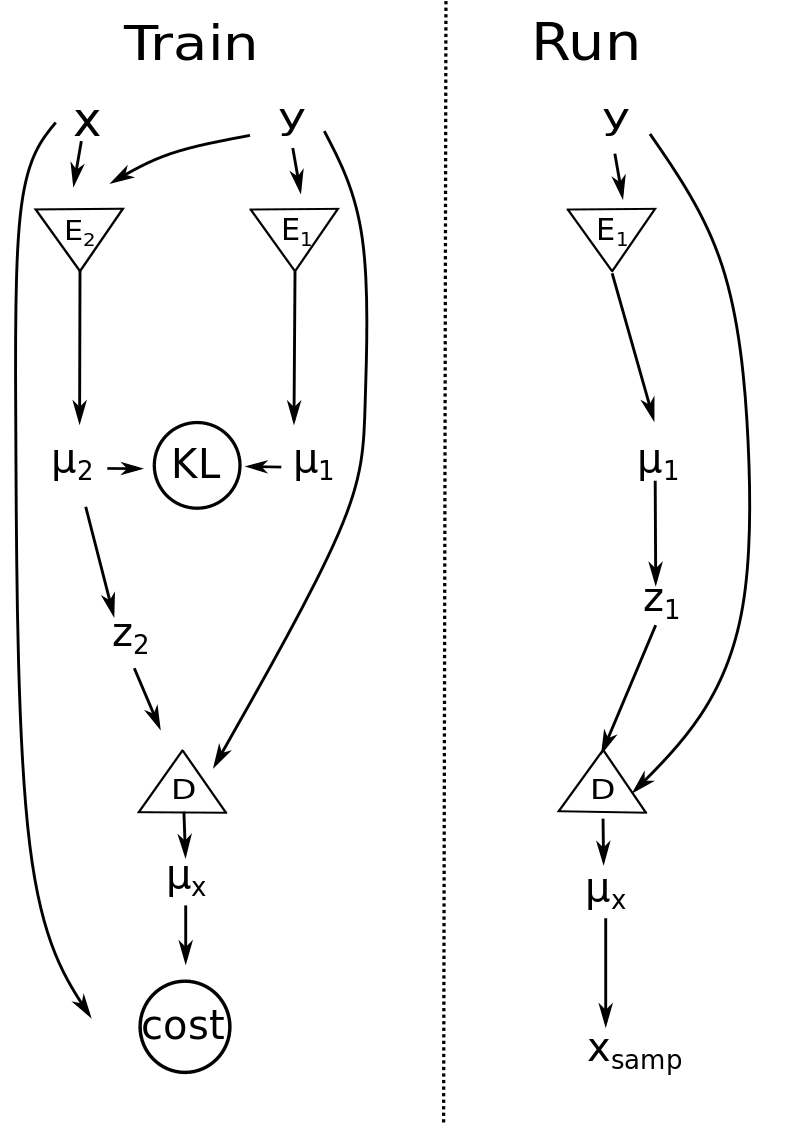
\includegraphics[width=\columnwidth]{images/network_setup.png}
    \caption{\label{fig:network_config}\chris{You are missing a crucial element
here. There should be an arrow from the y data to *both* encoders in the
training. Also, why have we made it so encoder 1 is on the right and encoder 2
is on the left. It reads weird.} This figure illustrates our neural network 
    training/testing operations. During training, a training set of GW signals ($y$) 
    and their corresponding true parameters ($x$) are given as input to encoder 
    networks $\textrm{E}_1$ and $\textrm{E}_2$. The KL divergence (Eq. \ref{eq:kl}) 
    is computed between mean latent space predictions from both encoder networks ($z^1_{\mu},z^2_{\mu}$)
    . $z^2_{\mu}$ is then summed togther with $z_{\log{(\sigma^{2})}} \cdot \epsilon(0,1)$ 
    and given as input to the decoder network. The decoder network predicts $x_{\mu}$ 
    and compares $x_{\mu}$ to the initial training parameters $x$ using Eq. \ref{eq:cost}. 
    After having trained our networks, we test using only $\textrm{E}_1$ and the decoder. 
    A set of test GW signals is given as input to $\textrm{E}_1$ in order to 
    produce a set of $z^1_{\mu}$ predictions. We apply Eq. \ref{eq:z_calc} to 
    get $z$ latent samples. Our $z$ latent space samples are given 
    as input to our decoder network along with our initial test GW signals 
    to get a set of $x_{\mu}$ predictions. We finally apply Eq. \ref{eq:x_calc} 
    to get a set of $x_\textrm{samp}$ samples.}
\end{figure}

%
% Training procedure
%
Training is performed through a series of 3 steps illustrated in \ref{fig:network_config}. 
In step 1 encoder-1 is given $y_t$ GW training samples and returns as output mean
latent space $z^{y}_{\mu}$. Then in step 2, encoder-2 takes a combination of $(x_{t},y_{t})$ 
and returns $z^{x,y}_{\mu}$. The K-L divergence between both $z^{y}_{\mu}$ and $z^{x,y}_{\mu}$ is 
computed and minimized in order to ensure that both distributions are consistent with each other. 
We finally sample from $z^{x,y}_{\mu}$ using a unitvariant Gaussian distribution 
in order to get a set of $z^{x,y}$ samples. These $z^{x,y}$ samples are combined with 
a set of $y_t$ training samples and fed as input to our decoder network, which attempts 
to reconstruct $x_t$ and outputs a mean predicted $x_{\mu}$. A cost function is then 
computed between $x_{\mu}$ and $x_t$ and is minimized.

%
% Brief introduction to loss functions used in the neural networks
%
In order for our variational autoencoders to learn anything, we need a metric by which 
we can assess the effectivness of our three networks. This is done by computing 
a loss function which minimizes the difference 
between predictions on the posterior with respect to the truth (cost function) and the Kullback-Leibler divergence 
between latent space distributions $z_1$ and $z_2$. 

%
% Cost function
%
The cost function is constructed by first defining a normalization factor

\begin{equation}
    f_{\textrm{norm}} = 0.5 \cdot \log(c + \exp(x_{\sigma})) - 0.5 \cdot \log(2\pi),
\end{equation}

where $c$ is a small constant and $x_{\sigma}$ are standard deviation predictions 
on the source paramters from the decoder network given latent space predictions 
from encoder-2 ($z_2$) and training GW sigals ($y_{t}$). We then 
compute 

\begin{equation}
    x_{\textrm{diff}} = (x^{z,y}_{\mu} - x_{\textrm{train}})^{2},
\end{equation}

where $x^{z,y}_{\mu}$ are the predicted mean parameters from the decoder network 
and $x_{\textrm{train}}$ are the true training parameters we are 
trying to predict. A Gaussian likelihood is computed and summed over

\begin{equation}
    \textrm{cost} = - \sum (-\frac{x_{\textrm{diff}}}{2c \cdot 
    x^{z^{x,y_{\textrm{train}}}_{\sigma},y_{\textrm{train}}}_{\sigma^{2}}} + f_{\textrm{norm}}),\label{eq:cost}
\end{equation}

where $x^{z^{x,y_{train}}_{\sigma},y_{train}}_{\sigma^{2}}$ are standard deviation squared predictions from the 
decoder network.


%
% KL divergence
%
The K-L divergence is computed in order to train 
encoder-1 and encoder-2 to produce consistant latent space 
distributions. This is done by computing 

\begin{equation}
    \begin{split}
    \textrm{KL-div} = \sum(\log{z^{y}_{\sigma}}-\log{z^{x,y}_{\sigma}} \\
    +\frac{\exp{(\log{z^{x,y}_{\sigma^{2}}+c)}}+(z^{x,y}_{\mu}-z^{y}_{\mu})^{2}}{2*\exp{(z^{y}_{\sigma^{2}}})}
    -\frac{1}{2}),\label{eq:kl}
    \end{split}
\end{equation}

where $z^{y}_{\sigma}$ is the predicted latent space standard deviation from $\textrm{E}_1$, 
$z^{x,y}_{\sigma}$ is the predicted latent space standard deviation from $\textrm{E}_2$, 
$c$ is a small constant, $z^{x,y}_{\sigma^{2}}$ is the predicted latent space 
standard deviation squared from $\textrm{E}_2$, $z^{y}_{\sigma^{2}}$ is the predicted 
latent space standard deviation squared from $\textrm{E}_1$, $z^{x,y}_{\mu}$ is the 
mean latent space from $\textrm{E}_2$ and $z^{y}_{\mu}$ is the mean latent space 
from $\textrm{E}_1$.

The mean of the summation in equation \ref{eq:cost}, $\overline{\textrm{cost}}$, 
is then summed together with the mean of the summation in equation \ref{eq:kl}, 
$\overline{\textrm{KL-div}}$ to 
get our final loss function

\begin{equation}
    \textrm{loss} = \overline{\textrm{KL-div}} + \overline{\textrm{cost}}.
\end{equation}

This loss is then backpropogated through all three networks 
(encoder-1, encoder-2, decoder) and repeated per batch of 
training samples for a pre-defined number of iterations. For our 
purposes, we found that $\sim3\textrm{e}6$ training iterations and 
a batch size of $128$ training samples were sufficient. A total 
of $1\textrm{e}6$ training samples were used. We additionally 
ensure that an inifinite number of noise realizations are effectively employed. This 
is done by adding a new unique set of random whitened noise to noise-free 
versions of our training samples for every new batch that the networks 
see. Each neural network is three layers deep, has $2048$ neurons, a latent 
space size of $64$ with $50\%$ dropout applied to each layer of each network.

%
% loss plot
%
\begin{figure}
    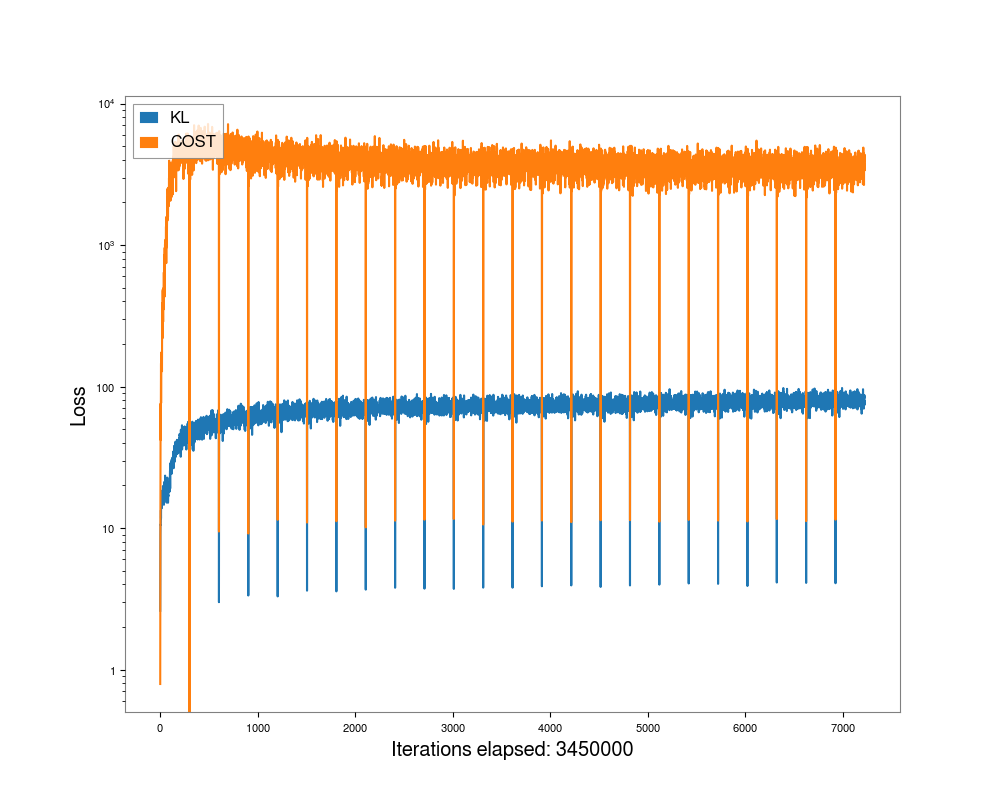
\includegraphics[width=\columnwidth]{images/losses_logscale.png}
    \caption{\label{fig:loss_log} Loss plot with the cost, KL, 
    and total loss values plotted as a function of the total 
    number of training iterations. We can conclude that our 
    neural networks have converged to their optimal state 
    when the slope of our loss curves are close to zero.}
\end{figure}

%
% Test procedure
%
After training has completed, we simply feed encoder-1 our test 
GW signals $y_{test}$. We take the output from encoder-1 $z^{y}_{\mu}$ 
and sample from a univariant Gaussian distribution in order to get 
a set of $z^{y}$ samples. Our $z^{y}$ samples are then combined with our 
test GW signals $y_{test}$ and fed as input to our pre-trained decoder 
network. The decoder network returns a set of mean $x_{\mu}$ predictions 
from which we sample from a Gaussian distribution in order to get 
our final posterior samples.

%
% Results
%
We present results from $25$ test cases of GWs produced from 
a parameter space which is consistent with the prior assumptions  
on the parameter space defined above. The only difference 
being that all of our time of coalescence parameters are fixed 
at $0.5s$ within the $1s$ time window. We compare our 
VAE predictions with posteriors produced by the Bilby
inference library.

%
% K-L divergence results
%
\begin{figure}
    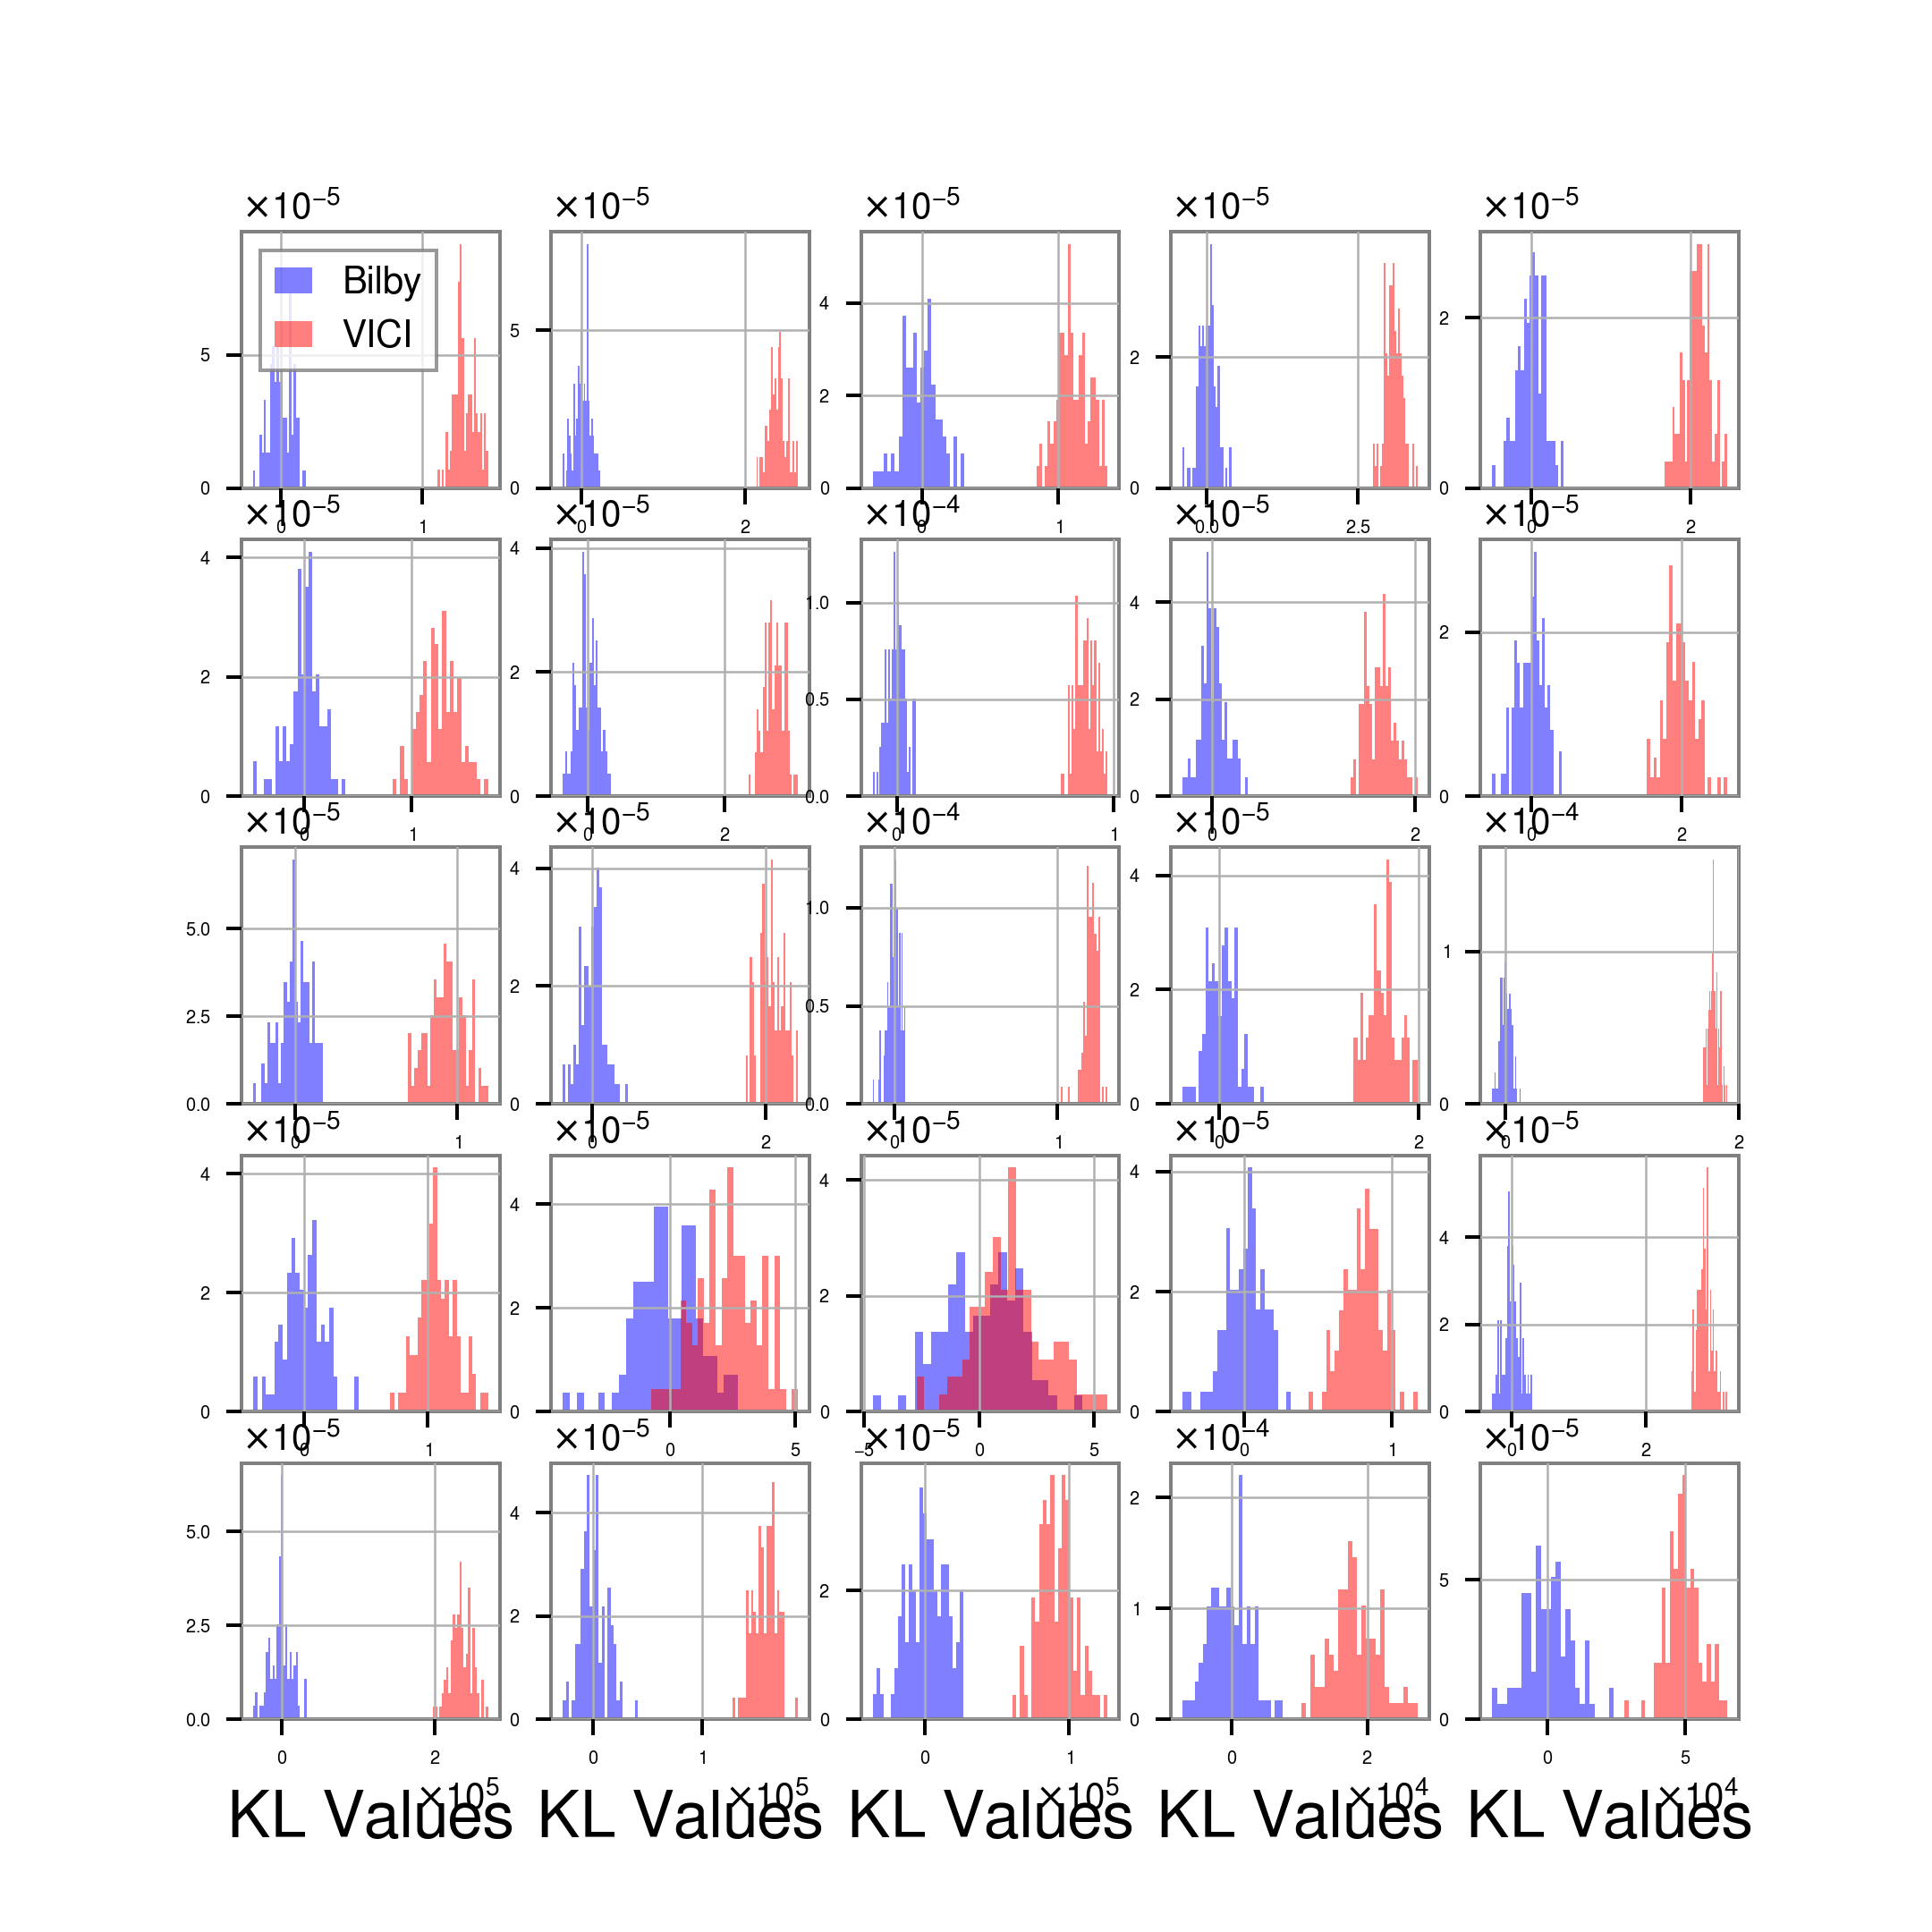
\includegraphics[width=\columnwidth]{images/hist-kl_0.png}
    \caption{\label{fig:kl_results} Histograms of 
    25 different test GW signal KL divergence values. 
    Red denotes predictions from the CVAE and blue 
    denotes predictions from Bilby.}
\end{figure}

In Fig. \ref{fig:kl_results} we show histograms of KL divergence 
values on $25$ test GW samples. The KL divergence is computed 
$100$ times per test sample through the initialization of random splits. We compute 
the KL divergence on CVAE results (red) by comparing CVAE predictions 
to Bilby predictions. Our benchmark Bilby (blue) results are computed by choosing 
random $50/50$ splits between results from the same bilby produced 
posterior. 


%
% A-D results
%
\begin{figure}
    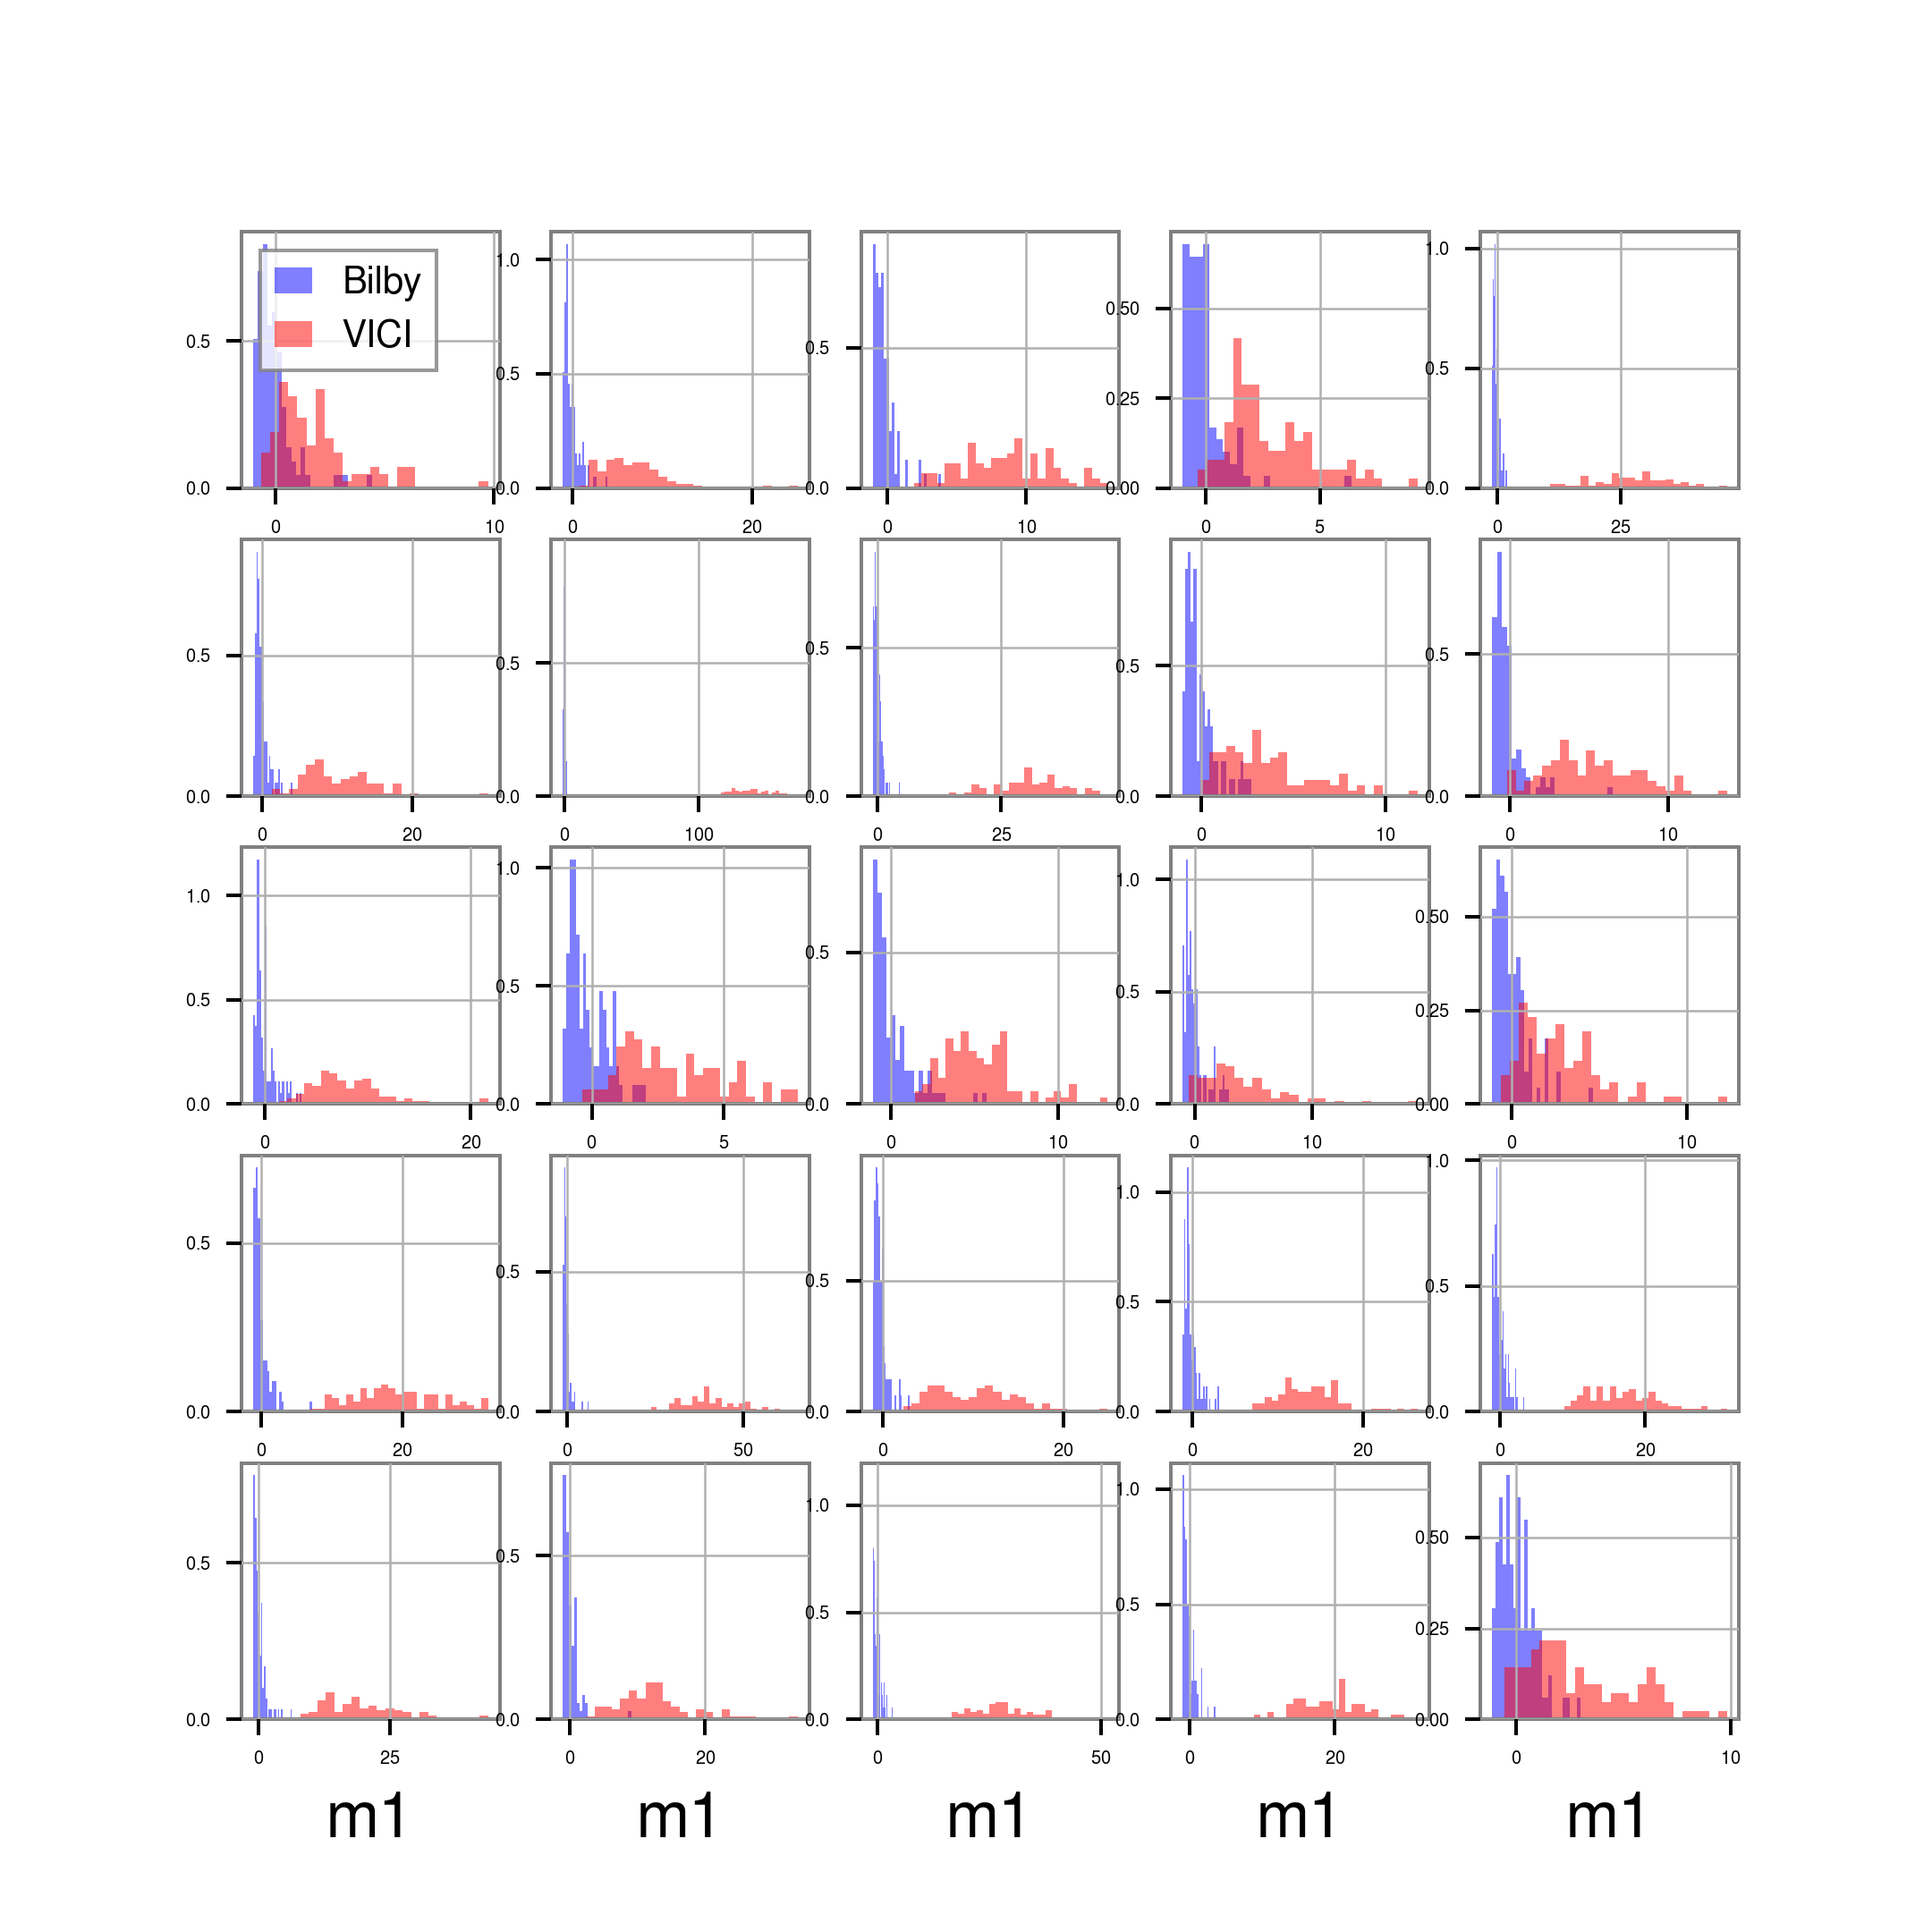
\includegraphics[width=\columnwidth]{images/hist-ad_0.png}
    \caption{\label{fig:ad_results} Histograms of 
    25 different test GW signal Anderson-Darling (AD) statistic 
    component mass 1 values. Distributions which are similar 
    will have AD values which are close to 0.
    Red denotes predictions from the CVAE and blue 
    denotes predictions from Bilby.}
\end{figure}

In Fig. \ref{fig:ad_results} we show histograms of AD 
statistic results computed over $100$ iterations per test sample. 
The AD statistic is a 1-dimensional figure of merit, 
so Fig. \ref{fig:ad_results} only illustrate results 
from predictions on $m_1$. The closer AD statistic 
values are to zero, the more likely that the two 
distributions being compared are drawn from 
the same distribution. As can be seen in Fig. \ref{fig:ad_results} 
there is some overlap between the machine learning 
predictions and our benchmark Bilby results.

%
% P-P plot
%
\begin{figure}
    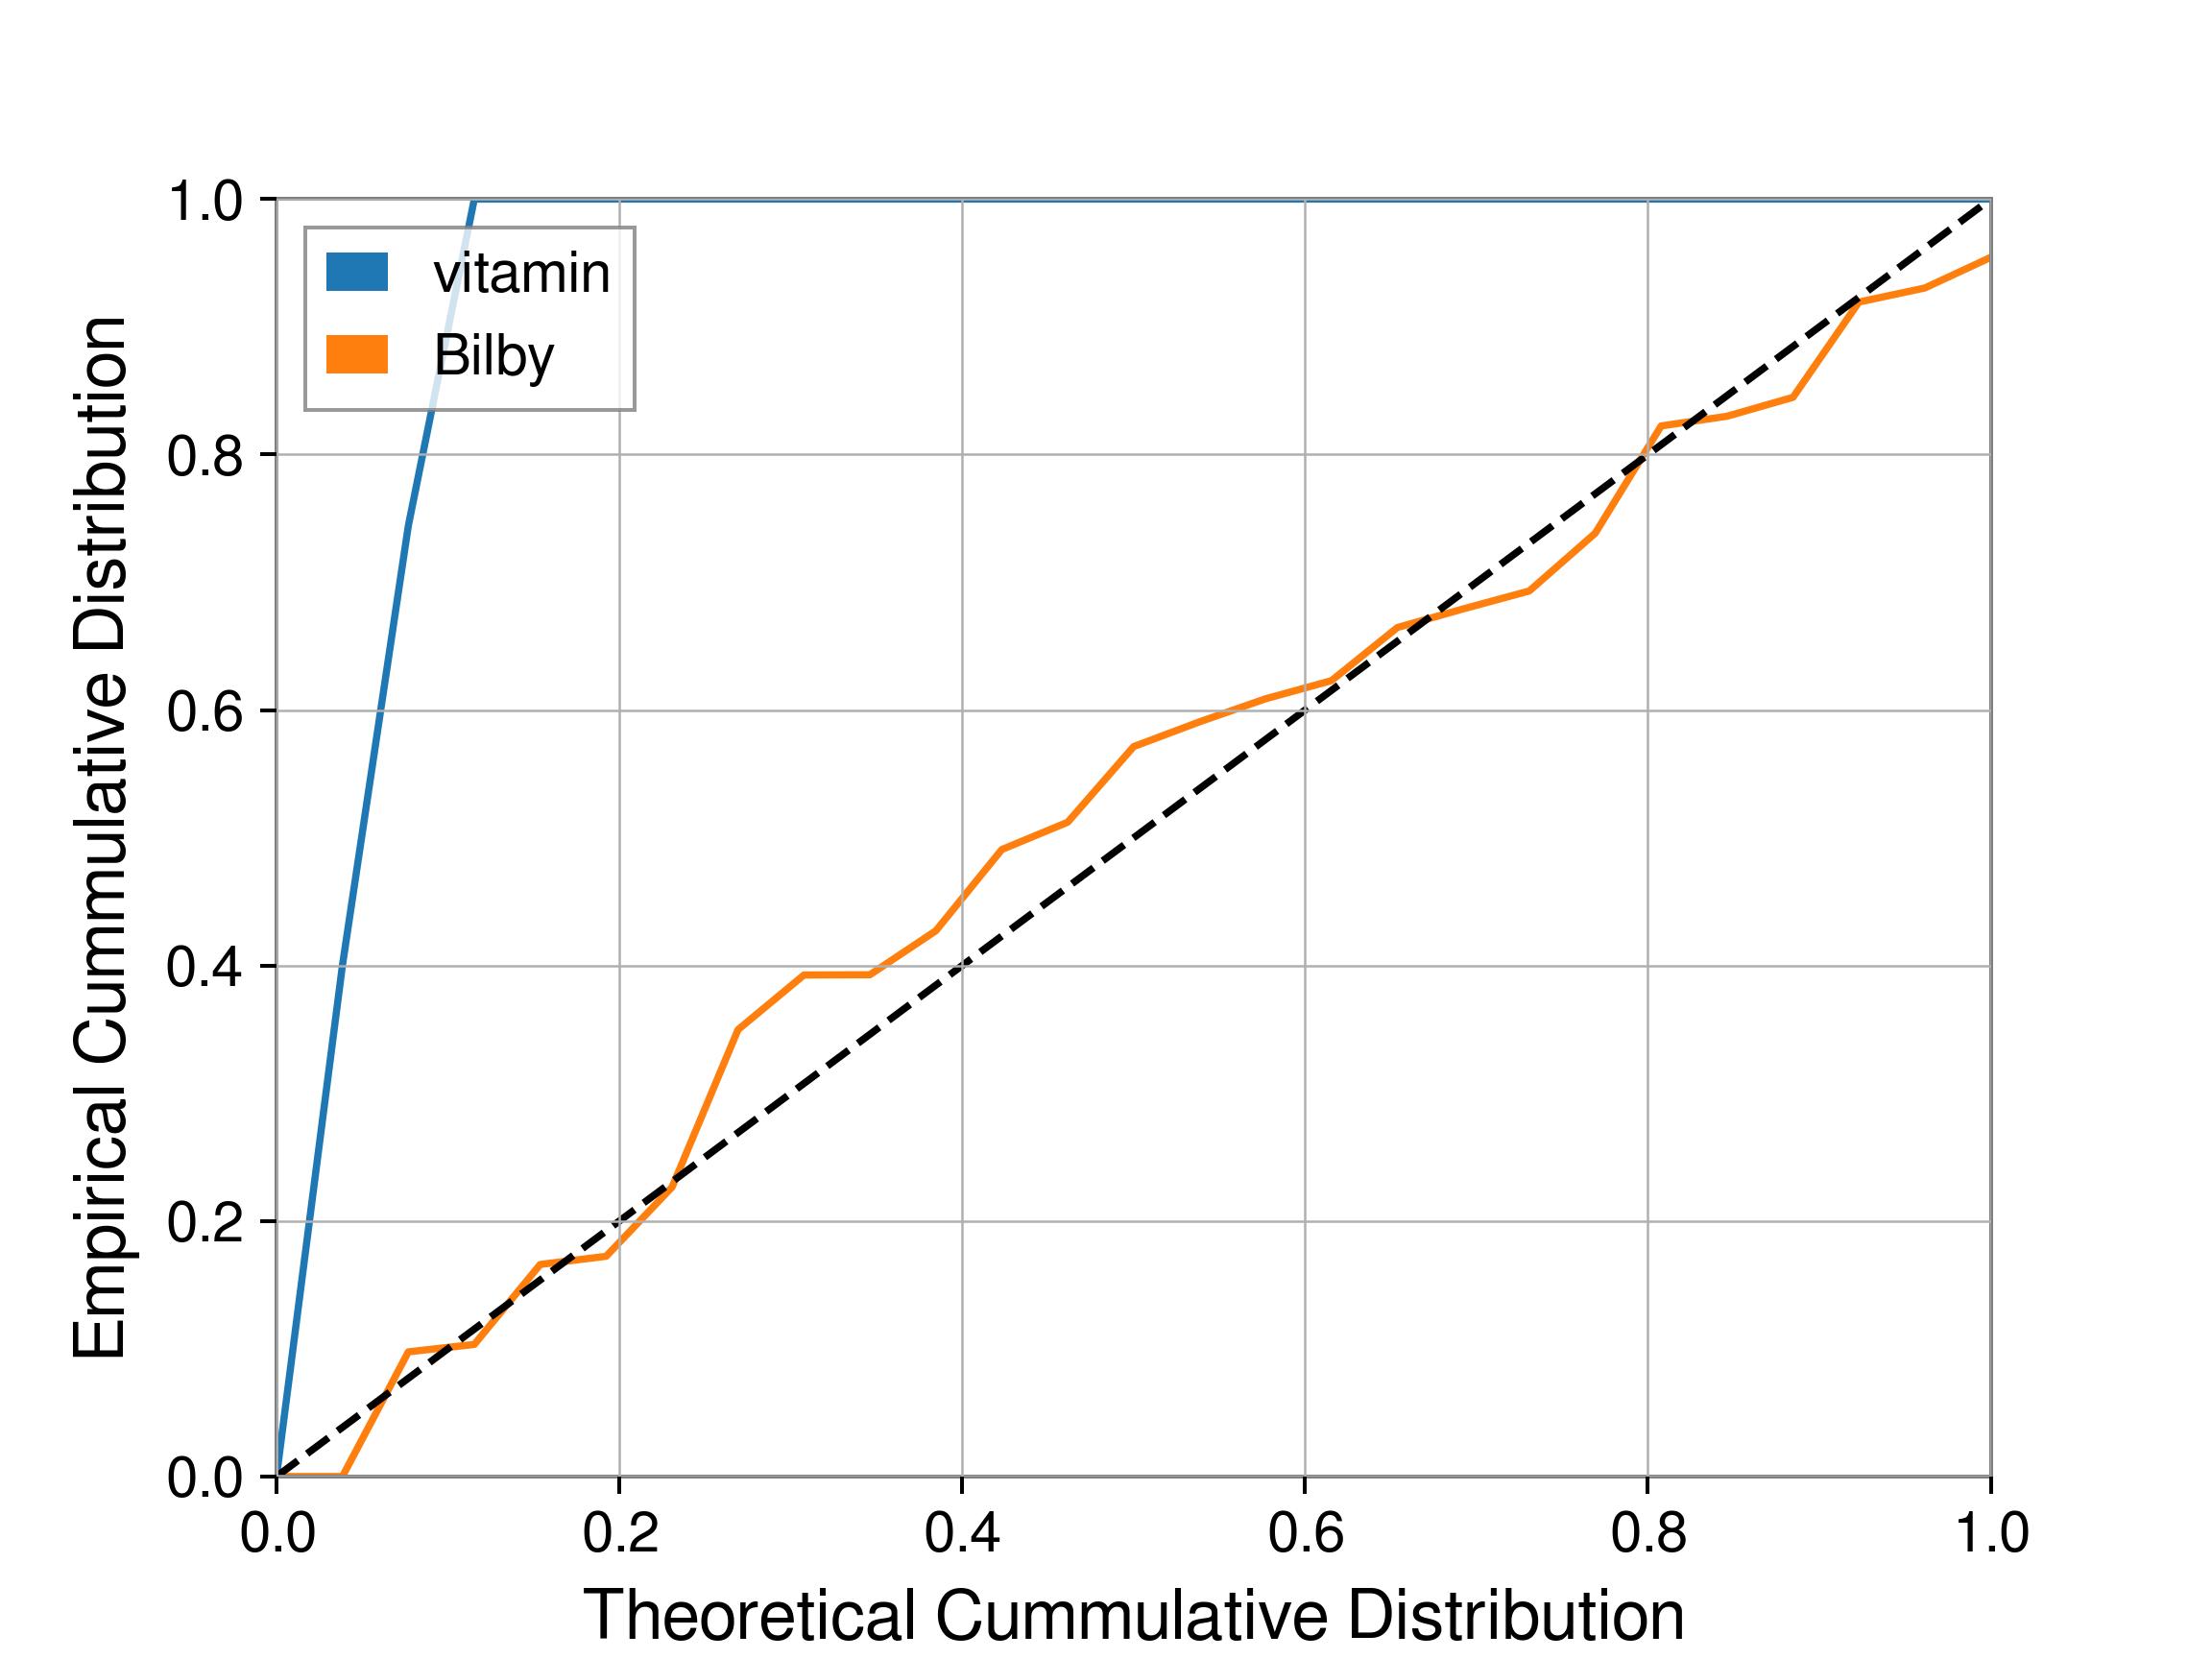
\includegraphics[width=\columnwidth]{images/latest_pp_plot.png}
    \caption{\label{fig:pp_plot} P-p plot 
    using $100$ unique test samples and $5000$
    posterior sample predictions per test sample. 
    The x axis denotes the theoretical cummulative 
    distribution whereas the y axis denotes 
    the predicted cummulative distribution.}
\end{figure}

In order to show that our results are consistent with the 
truth, we have additionally plotted probability-probability (p-p) 
plots in Fig. \ref{fig:pp_plot}. On the y axis is plotted the predicted 
cummulative distribution and on the x axis is plotted the theorectical 
distribution. Perfect alignment with the truth is illustrated by the 
black dashed diagonal line, while our empirical alignment is 
shown in the blue line. 

%
% 1-D overlap results
%
\begin{figure}
    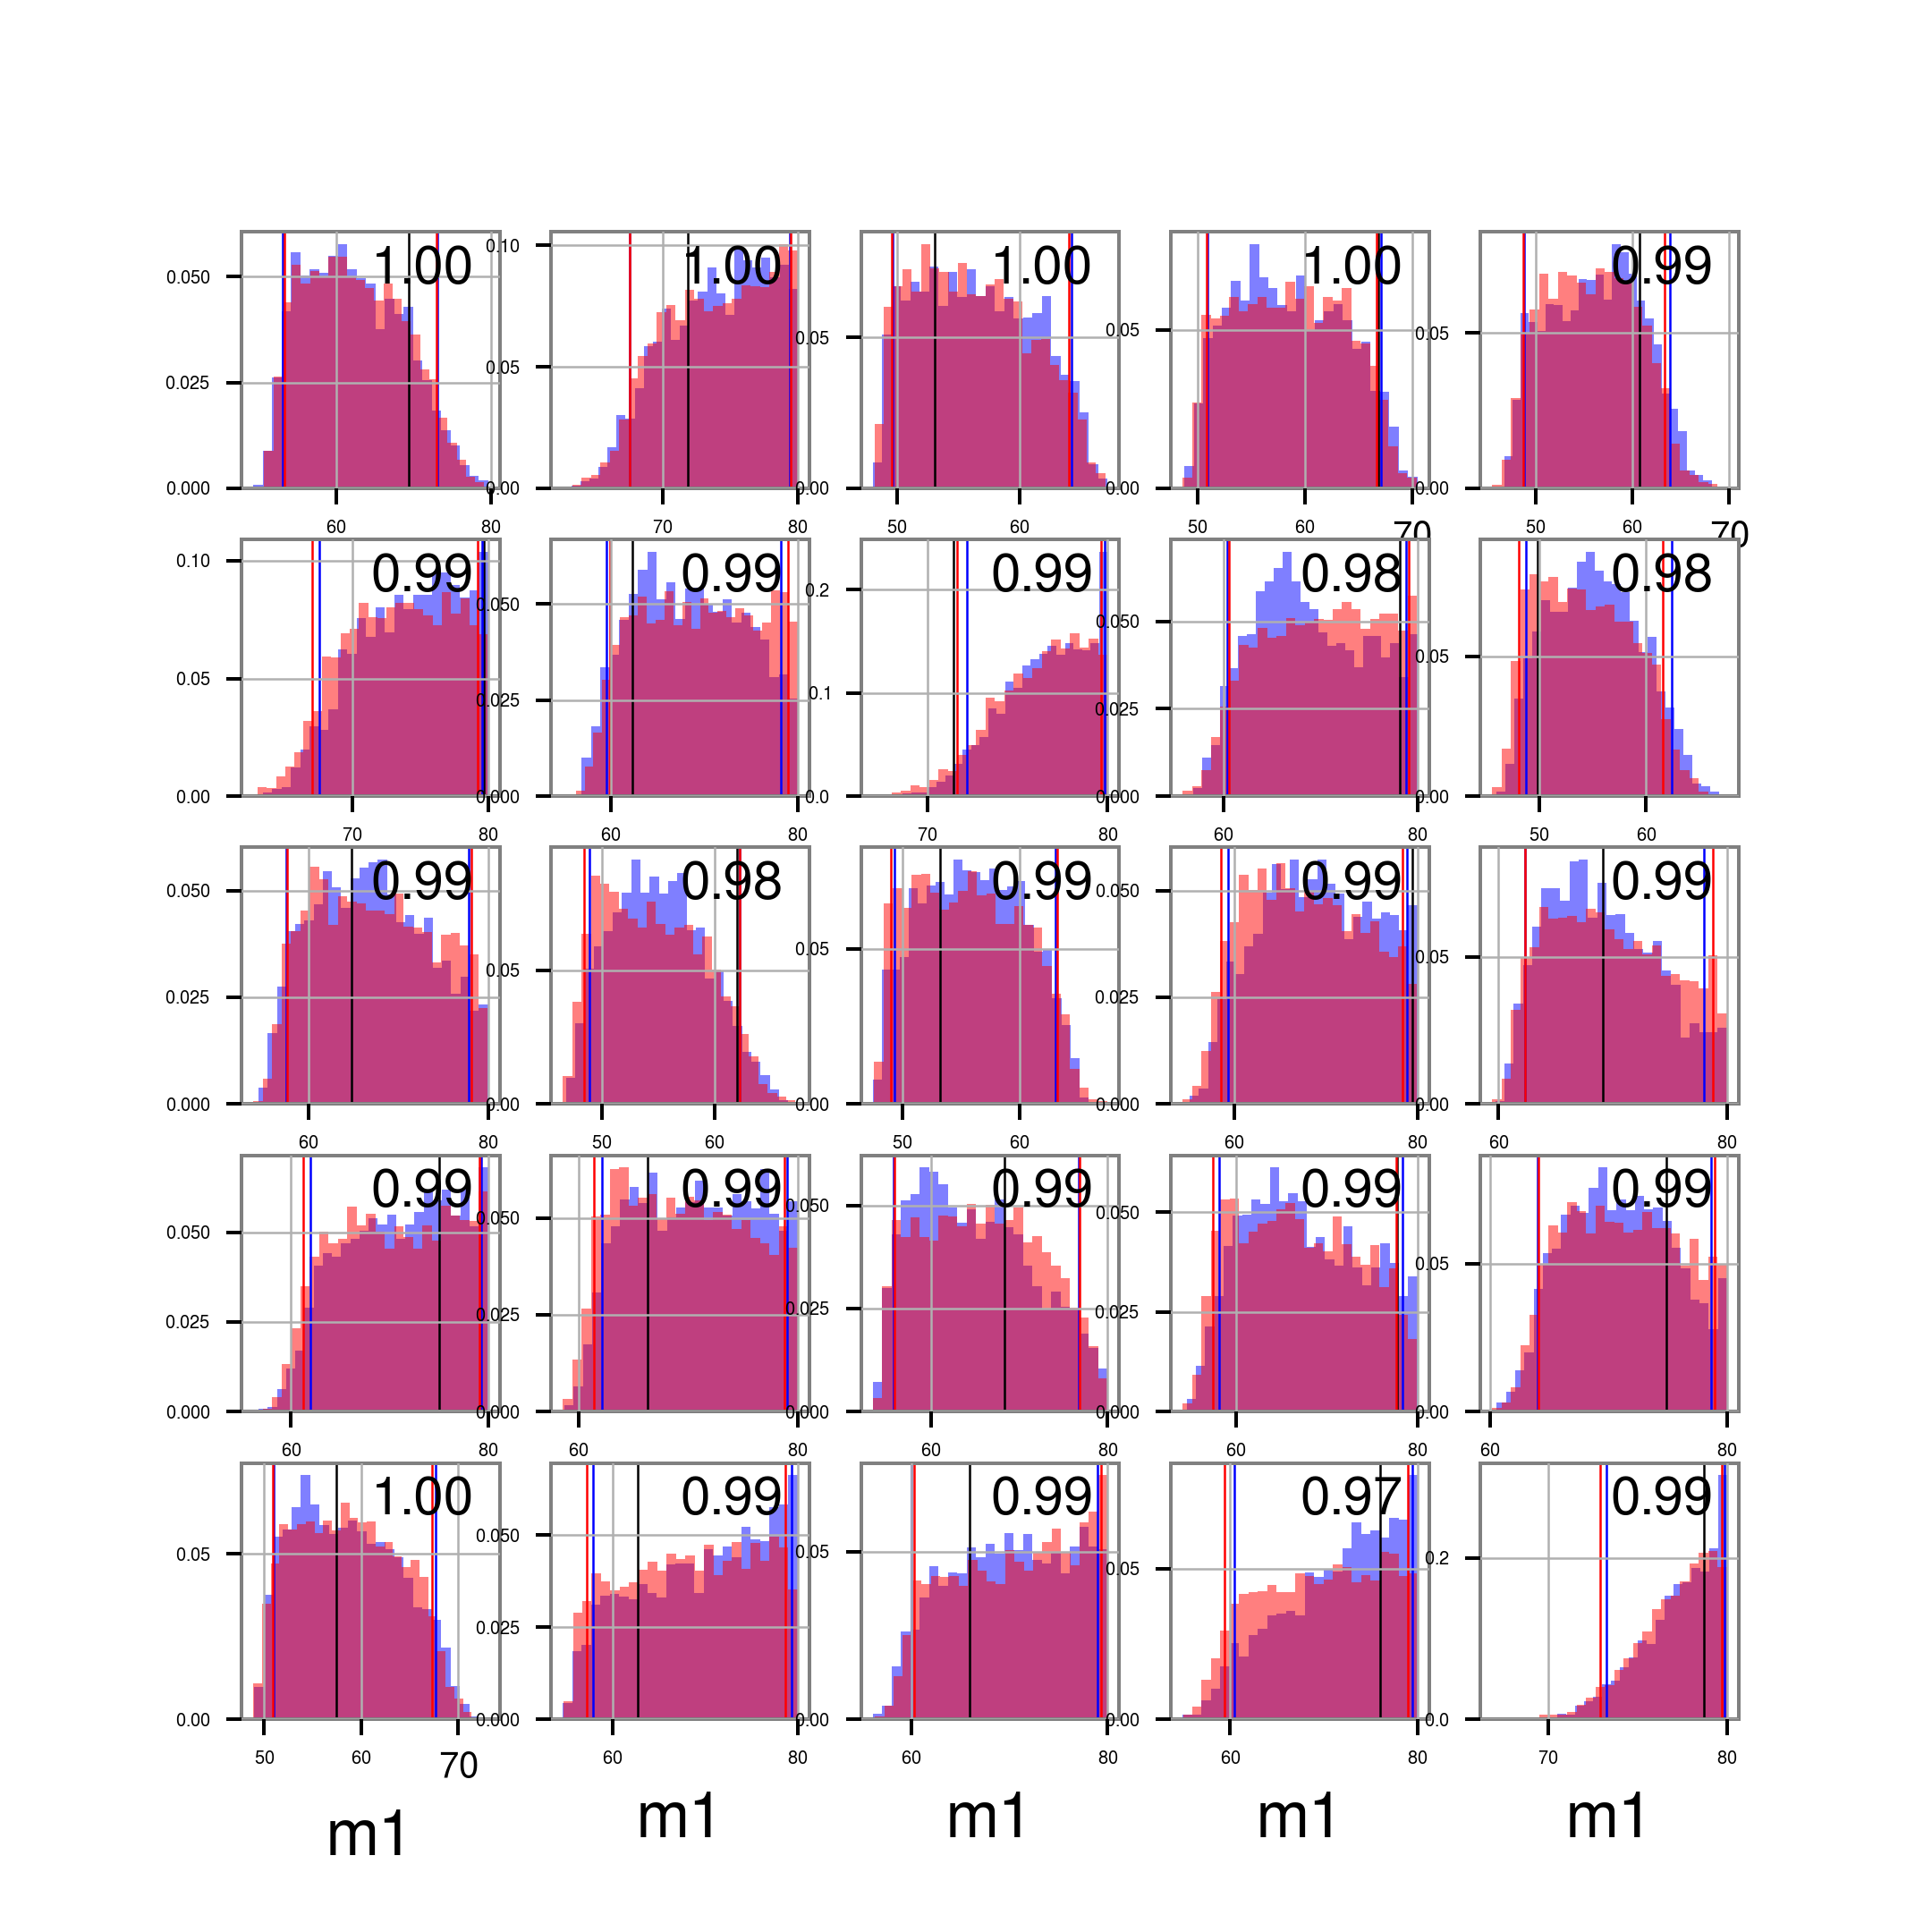
\includegraphics[width=\columnwidth]{images/latest-1d_0.png}
    \caption{\label{fig:1D_overlap} Histograms of 
    25 different test GW signal component mass 1 values. 
    Numbers in the upper right-hand corner denote overlap 
    values where 1 means $\sim{100}\%$ overlap and 0 
    means $\sim{0}\%$ overlap.
    Red denotes predictions from CVAE predictions and blue 
    denotes predictions from Bilby.}
\end{figure}

%
% 2D scatter plot
%
\begin{figure}
    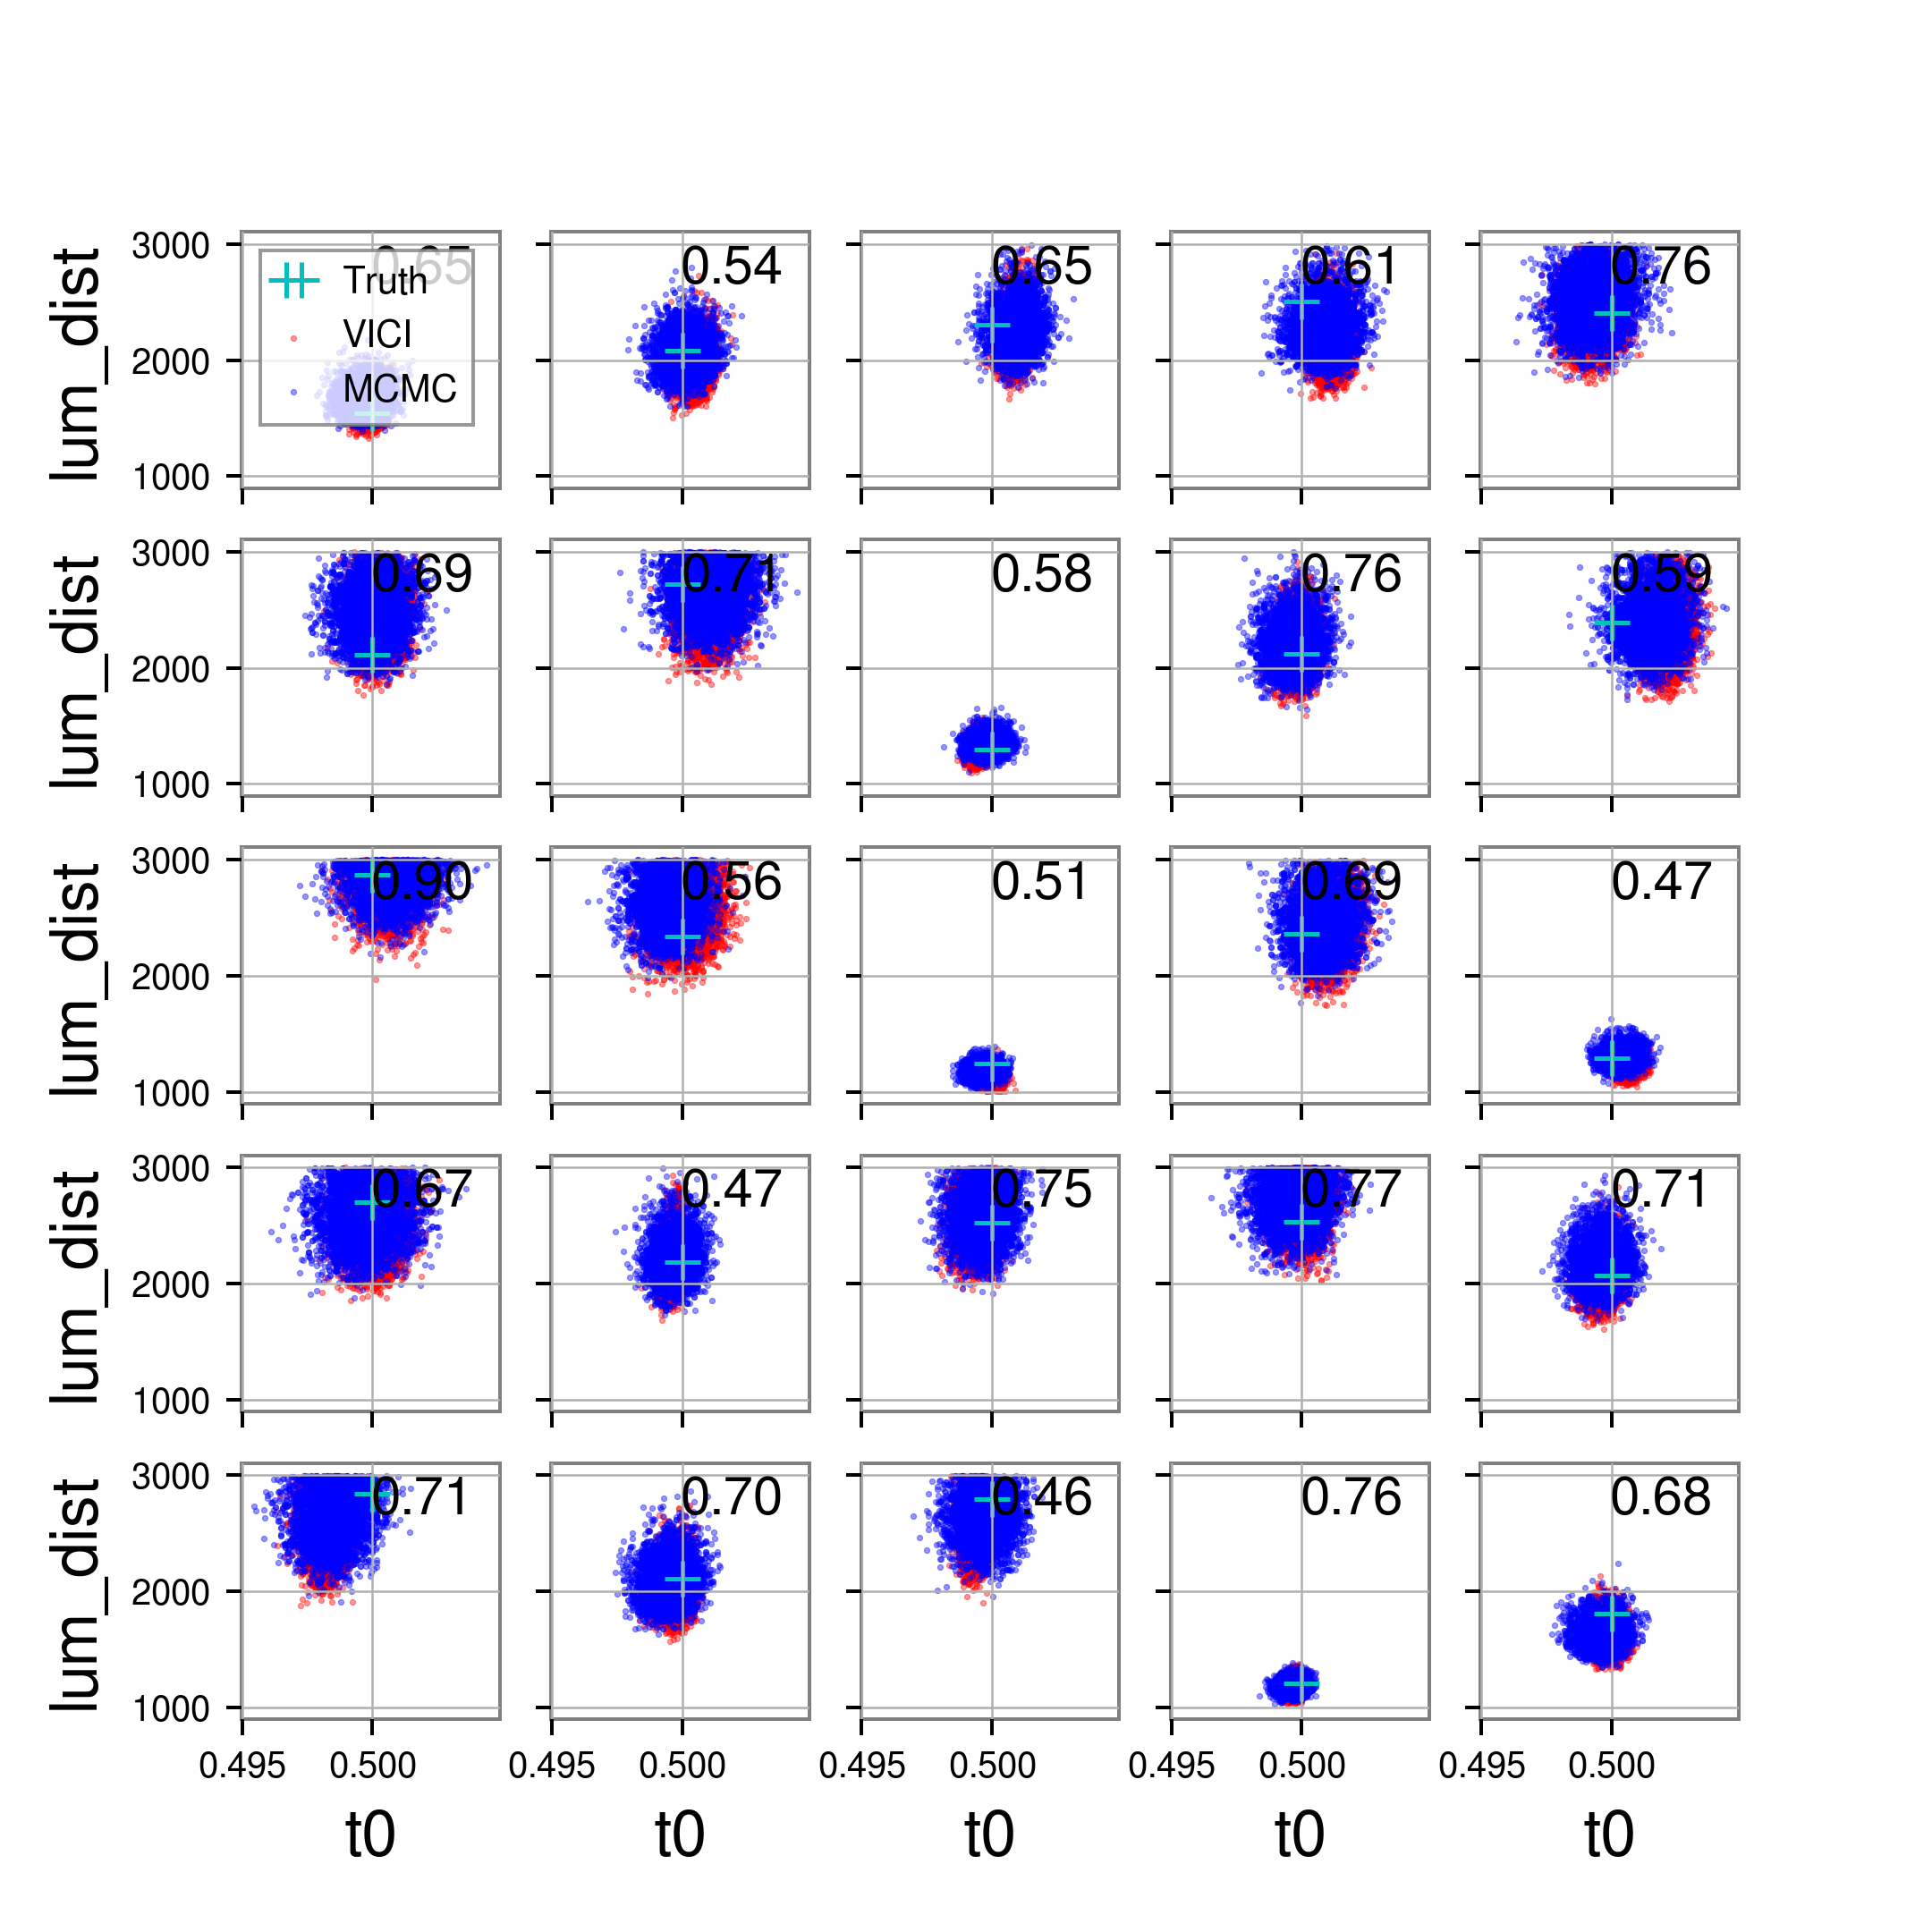
\includegraphics[width=\columnwidth]{images/posteriors_13.png}
    \caption{\label{fig:lum_dist-t0_scatter} This figure illustrates 
    25 different test GW samples with $5000$ posterior samples 
    from both Bilby and our CVAE plotted. Red denotes predictions 
    from the CVAE and blue denotes predictions from Bilby. Luminosity 
    distance is plotted as a function of time of coalescence with 
    4-dimensional overlap values printed in the upper right-hand 
    portion of each subplot.}
\end{figure}

We can further illustrate the accuracy of our machine 
learning predictions by directly plotting the samples 
generated by our CVAE and Bilby superimposed on each other. 
In Fig. \ref{fig:1D_overlap}, we histogram predictions sampled 
from the posterior through both Bilby (blue) and our CVAE (red). 
As can be clearly seen, the overlap between both Bilby and 
the CVAE is extremely high in the $m_1$ parameter space. Additional 
proof of high overlap between posteriors can also be seen 
in Fig. \ref{fig:lum_dist-t0_scatter} where 
we plot samples from both Bilby (blue) and the CVAE (red) posteriors 
with luminsoity distance as a function of $t_0$. 

%
% Conclusions
%
In this letter we have demonstrated that we 
are able to reproduce, to a high degree of accuracy, posteriors 
generated from Bayesian inference using machine learning. This 
is accomplished through the use of variational autoencoders 
trained on over 1 million whitened simulated gravitational 
wave signals. By building a neural network model which, 
when trained, can reproduce the true posterior in less than a 
second, we have demonstrated that neural networks 
can achieve the same sensitivity as that of Bayesian 
inference.

The significance of achieving similar sensitivities 
to Bayesian inference is most evident in the 
orders of magnitude speed-up in performance. The increase
in speed will help the LIGO-Virgo-Kagra calibration 
alert our electromagnetic follow-up partners with 
minimum latency.

Our work can further be expanded upon by including 
a variety of other GW sources such as Neutron star - 
black hole (NSBH) and binary neutron star (BNS) mergers 
at higher sampling frequencies. We have yet to demonstrate 
the effectivness of our method on additional parameters 
such as sky location and inclination angle, the benefits of which 
would be best realized in an end-to-end inference pipeline. 
Such a pipeline would be of great importance as the detectors 
increase up to their full potential design sensitivities.

\section{Methods}
Put methods in here.  If you are going to subsection it, use
\verb|\subsection| commands.  Methods section should be less than
800 words and if it is less than 200 words, it can be incorporated
into the main text.

\subsection{Method subsection.}

Here is a description of a specific method used.  Note that the
subsection heading ends with a full stop (period) and that the
command is \verb|\subsection{}| not \verb|\subsection*{}|.

\subsection{Loss function derivation}

This section is to be rephrased into appropriate language but for now I will
add my interpretation of the loss function and the design of the network.

We begin with the statement defining the aim of the analysis. We wish to obtain
a function that reproduces the posterior distribution (the probability of our
physical parameters given some measured data). We define the cross entropy
between 2 distributions as
%
\begin{equation}\label{eq:cross_ent}
H(p,r) = -\int dx\, p(x|y) \log r_{\theta}(x|y)
\end{equation}
%
where we have made the distributions explicitly conditional on $y$ (our
measurement). In this case $p(x|y)$ is the target distribution (the true
posterior) and $r_{\theta}(x|y)$ is the parametric distribution that we will
use neural networks to construct. In this case $\theta$ represents the
trainable neural network parameters. 

The cross-entropy is minimised when $p(x|y)=r_{\theta}(x|y)$ and so by maximising
%
\begin{equation}\label{eq:cost1}
C = \text{E}_{p(y)}\left[\int dx\,p(x|y) \log r_{\theta}(x|y)\right]
\end{equation}
% 
where $\text{E}_{p(y)}[\dot]$ indicates the expectation value over the
distribution of measurements, we therefore make the parameteric distribution as
similar to the target for all possible measurements $y$.

Converting the expectation value into an integral over $y$ weighted by $p(y)$
and applying Bayes theorem we obtain
%
\begin{equation}\label{eq:cost1}
C = \int dx\,p(x)\int dy\,p(y|x)\log r_{\theta}(x|y)
\end{equation}
%
where $p(x)$ is the prior distribution on the physical parameters $x$.

The conditional variational autoencoder network outlined in
Fig.~\ref{fig:network_config} makes use of a conditional latent variable model.
Our parameteric model is constructed from the product of 2 seperate
distributions marginalised over the latent space
%
\begin{equation}\label{eq:latent_model}
r_{\theta}(x|y) = \int dz\,r_{\theta_{1}}(z|y)r_{\theta_{2}}(x|z,y).
\end{equation}
%  
We have used $\theta_{1}$ and $\theta_{2}$ to indidate that the 2 seperate
networks modelling these distributions will be trained on these parameter sets
respectively. Both new conditional distributions are modelled as $n_{z}$
dimensional multivariate uncorrelated Gaussian distributions (governed by their
means and variances). However, this still allows $r_{\theta}(x|y)$ to take a
general form (although it does limit it to be unimodal).  

One could be forgiven in thinking that by setting up networks that simply aim
to maximise $C$ over the $\theta_{1}$ and $\theta_{2}$ would be enough to solve
this problem. However, as shown in~\cite{NIPS2015_5775} this is an intractable
problem and a network cannot be trained directly to do this. Instead we define
a recognition function $q_{\phi}(z|x,y)$ that will be used to derive an
\ac{ELBO}.

Let us first define the Kullback–Leibler divergence between 2 of our
distributions as
%
\begin{equation}\label{eq:kl}
\text{KL}\left[q_{\phi}(z|x,y)||r_{\theta_{2}}(z|x,y)\right] = \int dz\,
\log\left(\frac{q_{\phi}(z|x,y)}{r_{\theta_{2}}(z|x,y)}\right).
\end{equation}
%  
It can be shown that after some manipulation that
%
\begin{equation}\label{eq:elbo1}
\log r_{\theta}(x|y) = L + \text{KL}\left[q_{\phi}(z|x,y)||r_{\theta_{?}}(z|x,y)\right]
\end{equation}
%
where the \ac{ELBO} $L$ is given by
%
\begin{equation}\label{eq:elbo2}
L = \int dz\,
q_{\phi}(z|x,y)\log\left(\frac{r_{\theta_{2}}(x|z,y)r_{\theta_{1}}(z|y)}{q_{\phi}(z|x,y)}\right)
\end{equation}
%
and is so-named since $\text{KL}$ cannot be negative and has a minimum of zero.
Therefore, if we were to find a $q_{\phi}(z|x,y)$ function (optimised on
$\phi$) that minimised the KL-divergence then we can state that
%
\begin{equation}
\log r_{\theta}(x|y) \geq L.
\end{equation}
%
After some further manipulation of Eq.\ref{eq:elbo2} we find that
%
\begin{align}\label{eq:logr}
\log r_{\theta}(x|y) \geq & \text{E}_{q_{\phi}(z|x,y)}\left[\log
r_{\theta_{2}}(x|z,y)\right] \nonumber\\
&-\text{KL}\left[q_{\phi}(z|x,y)||r_{\theta_{1}}(z|y)\right].
\end{align}
%
We can now substitute this inequality into Eq.~\ref{eq:cost1} (our cost
function) to obtain
%
\begin{align}\label{eq:cost2}
C \geq & \int dx\, p(x)\int dy\,p(y|x)
\left[\text{E}_{q_{\phi}(z|x,y)}\left[\log r_{\theta_{2}}(x|z,y)\right]
\right.\nonumber\\
&-\left.\text{KL}\left[q_{\phi}(z|x,y)||r_{\theta_{1}}(z|y)\right]\right]  
\end{align}
%
which can in practice be approximated as a stochastic integral over draws of
$x$ from the prior, $y$ from the likelihood function $p(y|x)$, and from the
recognition function, giving us
%
\begin{align}\label{eq:cost3}
C \geq & \frac{1}{N}\sum_{n=1}^{N}\left[\log
r_{\theta_{2}}(x_{n}|z_{n},y_{n})\right.\nonumber\\
&\left.-\text{KL}\left[q_{\phi}(z|x_{n},y_{n})||r_{\theta_{1}}(z|y_{n})\right]\right].
\end{align}
% 
In this case we draw $N$ sets of physical parameter, corresponding data
sets, and draws from the recognition function. It is important to note that
whilst it is true that the KL-divergence between the $q_{\phi}(z|x,y)$ and
$r_{\theta_{2}}(z|x,y)$ (seen in Eq.~\ref{eq:elbo1}) should be minimised and in
an ideal case be equal to zero, that is not the case for the KL-divergence in
Eq.~\ref{eq:cost3}. In this case our aim is to maximise $C$ which implies that
the KL-divergence should be low but not necessarily zero.

We have now set up a system composed of 3 functions that have well defined
inputs and outputs where the mapping of those inputs to outputs is governed by
the parameter sets $\theta_{1},\theta_{2},\phi$. These parameters are the
weights and biases of 3 neural networks acting as (variational) encoder,
decoder, and encoder respectively. To train such a network one must connect the
inputs and outputs appropriately to compute $C$ and back-propogate cost
function derivatives to update the network parameters. The network structure
shown in Fig.~\ref{fig:network_config} shows how for a batch of $N$ sets of $x$
and corresponding $y$ values first both $x$ and $y$ are fed into the encoder 2
network that produces the means and variances of the latent space $z$
describing the $q_{\phi}(z|x,y)$ distribution function. Next (the order does
not matter) the data $y$ alone is passed into the encoder 1 network that
produces the means and variances of the latent space $z$ describing the
$r_{\theta_{1}}(z|y)$ distribution function. Given the parameters of these
Gaussian (diagonal covariance matrix) distributions the $\text{KL}$-divergence
is computed as
%
\begin{align}\label{eq:klgauss}
\text{KL}\left[q_{\phi}(z|x_{n},y_{n})||r_{\theta_{1}}(z|y_{n})\right] =&
\frac{1}{2}\sum_{j=1}^{n_{z}}\left[\frac{\sigma_{q,j}^{2}}{\sigma_{r,j}^{2}} +
\frac{(\mu_{r,j}-\mu_{q,j})^{2}}{\sigma_{r,j}^{2}}\right.\nonumber\\ 
&\left.+
\log\left(\frac{\sigma_{r,j}^{2}}{\sigma_{q,j}^{2}}\right)\right] -
\frac{n_{z}}{2}
\end{align}
%
where those labelled and indexed parameters output from the encoder networks
are denoted by $\mu$ and $\sigma$.

To evaluate the first term within the loss function (Eq.~\ref{eq:cost3}) we
require the data $y$ and a randomly drawn $z$ value from the latent space defined
by $q_{\phi}(z|x,y)$. These are then passed as input into the decoder network D
that produces the means and variances in the physical parameter space $x$ describing
the $r_{\theta_{2}}(x|z,y)$ distribution function. With the function now well
defined we simply evaluate the function at the values of the input $x_{n}$
values. Training of the network proceeds until a convergence of the cost is
seen. 

When the network has been trained it can be used for the inference of unknown
physical parameters given a new single instance of measured data $y$. To do
this one is interested in obtaining samples from the distribution
$r_{\theta}(x|y)$ which can be obtained by evaluating
Eq.~\ref{eq:latent_model}. To do this using the network we first obtain the
parameters governing the function $r_{\theta_{1}}(z|y)$ by passing the data $y$
into the encoder 1 network. Using the output means and variances on the latent space
$z$ we then draw from that space to obtain a random latent space realisation.
This $z$ value and the original $y$ data is then input into the decoder network
which outputs the mean and variance parameters governing the function
$r_{\theta_{2}}(x|z,y)$. The next step is to draw a random $x$ realisation from
that function. This is representative of a posterior sample from the target
distribution $p(x|y)$ and to obtain an informative description of the entire
distribution one would repeat the procedure with the same input data
$\mathcal{O}(1000)$ times from which parameter confidence bounds can be
determined.      


%
% acknowledge people and funding agencies
%
\section{Acknowledgements.}
%
We would like to acknowledge valuable input from the LIGO-Virgo Collaboration
specifically from {\textbf{someone}}, and the parameter estimation and
machine-learning working groups. The authors also gratefully acknowledge the
Science and Technology Facilities Council of the United Kingdom. CM and SH are
supported by the Science and Technology Research Council (grant
No.~ST/~L000946/1) and the European Cooperation in Science and Technology
(COST) action CA17137.

%% Here is the endmatter stuff: Supplementary Info, etc.
%% Use \item's to separate, default label is "Acknowledgements"

%\begin{addendum}
% \item Put acknowledgements here.
% \item[Competing Interests] The authors declare that they have no
%competing financial interests.
% \item[Correspondence] Correspondence and requests for materials
%should be addressed to Hunter Gabbard~(email: h.gabbard.1@research.gla.ac.uk).
%\end{addendum}

\bibliographystyle{apsrev4-1}
\bibliography{references}% Produces the bibliography via BibTeX.

\end{document}
